%   Switch the contents entries from "Chapter" to "Appendix". Written from
%   inside the first appendix file so it lands in the contents BEFORE this
%   chapter's entry (\include writes each file's entries separately).
\addtocontents{toc}{\protect\renewcommand{\protect\cftchappresnum}{\appendixname\space}}
\chapter{Additional Control Simulation Results}
\label{app:control-results}
 
This appendix supports Chapter~\ref{ch:theory}. Section~\ref{app:model-parameters} gives the parameter values used in the models, and Sections~\ref{app:temp-control-sim} and~\ref{app:co2-control-sim} give the simulation models and extra results for the controller design.

%*********************************************************************
%   APPENDIX: MODEL PARAMETER ESTIMATES
%   Belongs to Chapter 3, Theoretical development.
%   Referenced from Sections 3.1.2, 3.1.3 and 3.2.2 as app:model-parameters.
%*********************************************************************
\section{Model Parameter Estimates}
\label{app:model-parameters}

The values below were used in the thermal and CO\textsubscript{2} models in Chapter~\ref{ch:theory}. They are all estimates made before the chamber was built, and they were replaced by measured values in Chapter~\ref{ch:thermalID}.

\subsection{Thermal Parameters}
\label{app:thermal-parameters}

\begin{table}[H]
    \centering
    \caption[Thermal parameter values]{\textbf{Parameter values used in the chamber model.}}
    \label{tab:thermal-params}
    \small
    \setlength{\tabcolsep}{6pt}
    \renewcommand{\arraystretch}{1.2}
    \begin{tabular}{@{}>{\raggedright\arraybackslash}p{1.6cm}>{\raggedright\arraybackslash}p{3.0cm}>{\raggedright\arraybackslash}p{8.4cm}@{}}
        \toprule
        \textbf{Symbol} & \textbf{Value} & \textbf{Description} \\
        \midrule
        $h_c$ & 5\,W/m\textsuperscript{2}K & Natural convection, surfaces facing the enclosed chamber \citep{incropera_fundamentals_2007} \\
        $h_a$ & 8\,W/m\textsuperscript{2}K & Natural convection and radiation combined, outer surfaces \citep{incropera_fundamentals_2007} \\
        $k_w$ & 0.07\,W/mK & Effective conductivity of the printed PETG wall \\
        $t_w$ & 3\,mm & Wall thickness \\
        $k_p$ & 0.13\,W/mK & Polystyrene plate base \\
        $t_p$ & 1\,mm & Plate base thickness \\
        $A_w$ & 0.0604\,m\textsuperscript{2} & Plain wall area \\
        $A_g$ & 0.0168\,m\textsuperscript{2} & Glass area \\
        $A_p$ & 0.0109\,m\textsuperscript{2} & Plate area \\
        $P_h$ & 36\,W & Three film heaters at 12\,W each \\
        $\rho_{air}$, $c_{p,air}$ & 1.2\,kg/m\textsuperscript{3}, 1005\,J/kgK & Chamber air \\
        $\rho_{w}$, $c_{p,w}$ & 1270\,kg/m\textsuperscript{3}, 1200\,J/kgK & Solid PETG \\
        \bottomrule
    \end{tabular}
\end{table}

Two convection coefficients are used because the inside and outside surfaces are in different conditions. Radiation from the outside surfaces is not modelled on its own, so $h_a$ is taken at the upper end of its range to cover both convection and radiation. The wall conductivity had to be estimated because a printed wall is not solid. Its outer faces are solid, but the core is printed at 10 to 30\% infill, so it is mostly air. The value therefore lies between still air (0.025\,W/mK) and solid PETG (about 0.2\,W/mK), and 0.07\,W/mK was used.

\paragraph{Resistances.}
Heat leaving through the wall or the plate passes through three resistances in series: convection from the air to the inside surface, conduction through the material, and convection from the outside surface to the room. Series resistances add, with $R_{cond} = t/kA$ and $R_{conv} = 1/hA$. The glass path has only the first of these, since the glass is its own node in the model. This gives

\begin{align}
R_{ca} &= \frac{1}{h_c A_w} + \frac{t_w}{k_w A_w} + \frac{1}{h_a A_w} = 3.31 + 0.710 + 2.07 = 6.09\,\text{K/W}, \label{eq:rca} \\[4pt]
R_{cg} &= \frac{1}{h_c A_g} = 11.9\,\text{K/W}, \label{eq:rcg} \\[4pt]
R_{cp} &= \frac{1}{h_c A_p} + \frac{t_p}{k_p A_p} + \frac{1}{h_a A_p} = 18.35 + 0.706 + 11.47 = 30.52\,\text{K/W}. \label{eq:rcp}
\end{align}

\paragraph{Capacitance.}
Thermal capacitance is the energy needed to raise a body by one degree, $C = \rho V c_p$. The chamber air on its own gives only 1.2\,J/K. The printed wall stores far more heat, so it was included in the chamber capacitance. A solid wall would store 276\,J/K, but only about 60\% of the printed wall is plastic, which gives 166\,J/K. The chamber capacitance is therefore $C_c = 1.2 + 166 \approx 167$\,J/K.

Including the whole wall is an approximation. The wall sits between the chamber and room temperatures, so it does not warm fully with the air, and the model was expected to overestimate the time constant. The model was only used for the first controller tuning.

\begin{table}[H]
    \centering
    \caption[Glass model parameters]{\textbf{Parameter values used in the glass model.}}
    \label{tab:glass-params}
    \small
    \setlength{\tabcolsep}{6pt}
    \renewcommand{\arraystretch}{1.2}
    \begin{tabular}{@{}>{\raggedright\arraybackslash}p{1.6cm}>{\raggedright\arraybackslash}p{2.4cm}>{\raggedright\arraybackslash}p{9.0cm}@{}}
        \toprule
        \textbf{Symbol} & \textbf{Value} & \textbf{Description} \\
        \midrule
        $R_{cg}$ & 11.9\,K/W & Glass to chamber air, the same path as Equation~\ref{eq:rcg} seen from the other side \\
        $R_{ga}$ & 7.4\,K/W & Glass to room, a single convection step, $1/(h_a A_g)$ \\
        $R_{tot,g}$ & 4.56\,K/W & The two above in parallel \\
        $C_g$ & 34.7\,J/K & $\rho V c_p$ for the 150 $\times$ 112 $\times$ 1.1\,mm pane, soda lime glass at 2500\,kg/m\textsuperscript{3} and 750\,J/kgK \\
        $P_g$ & 16\,W & ITO coating at 12\,V, nominal within a 10.7 to 21.5\,W range \\
        \bottomrule
    \end{tabular}
\end{table}

\subsection{CO\textsubscript{2} Parameters}
\label{app:co2-parameters}

\begin{table}[H]
    \centering
    \caption[CO\textsubscript{2} model parameters]{\textbf{Parameter values used in the CO\textsubscript{2} model.} $Q_{in}$ is a design value and $Q_L$ is an assumption that still needs to be measured.}
    \label{tab:co2-parameters}
    \small
    \setlength{\tabcolsep}{6pt}
    \renewcommand{\arraystretch}{1.2}
    \begin{tabular}{@{}>{\raggedright\arraybackslash}p{1.6cm}>{\raggedright\arraybackslash}p{2.6cm}>{\raggedright\arraybackslash}p{8.8cm}@{}}
        \toprule
        \textbf{Symbol} & \textbf{Value} & \textbf{Description} \\
        \midrule
        $V$ & 0.99\,L & Free gas volume, from the chamber dimensions in Section~\ref{subsec:modelling-approach}, before the plate and fittings \\
        $\chi_s$ & 1.0 & Supply gas, treated as pure since bottled CO\textsubscript{2} is typically above 99.9\% \\
        $\chi_a$ & 0.0004 & Room air, 400\,ppm \\
        $\chi_0$ & 0.05 & Operating point, 5\% \\
        $Q_{in}$ & 0.1\,L/min & Regulator flow with the solenoid open, a design target \\
        $Q_L$ & $5.5\times10^{-4}$\,L/s & Leak exchange flow, assumed 2 air changes per hour \\
        $\mu_0$ & 1.7\% & Steady duty at the operating point \\
        \bottomrule
    \end{tabular}
\end{table}

Setting Equation~\ref{eq:co2-balance} to zero gives the duty needed to hold 5\% against the assumed leak,
$\mu_0 = Q_L(\chi_0-\chi_a) / Q_{in}(\chi_s-\chi_0) = 1.7\%$.

 
\section{Temperature Control}
\label{app:temp-control-sim}

This section supports Section~\ref{subsec:temperature-control}. Figure~\ref{fig_T1_simulink} shows the Simulink model of the two temperature loops. Figures~\ref{fig_T4_setpoint_weighting} and~\ref{fig_T5_ambient_disturbances} show the effect of setpoint weighting and of changes in room temperature. Figures~\ref{fig_T6_robustness} to~\ref{fig_T9_discrete_vs_continuous} check the design against model error, coupling between the loops, added delay and the 1\,s sample time. All of these use the estimated parameters, from before the plant was measured in Chapter~\ref{ch:thermalID}.

\begin{figure}[htbp]
    \centering
    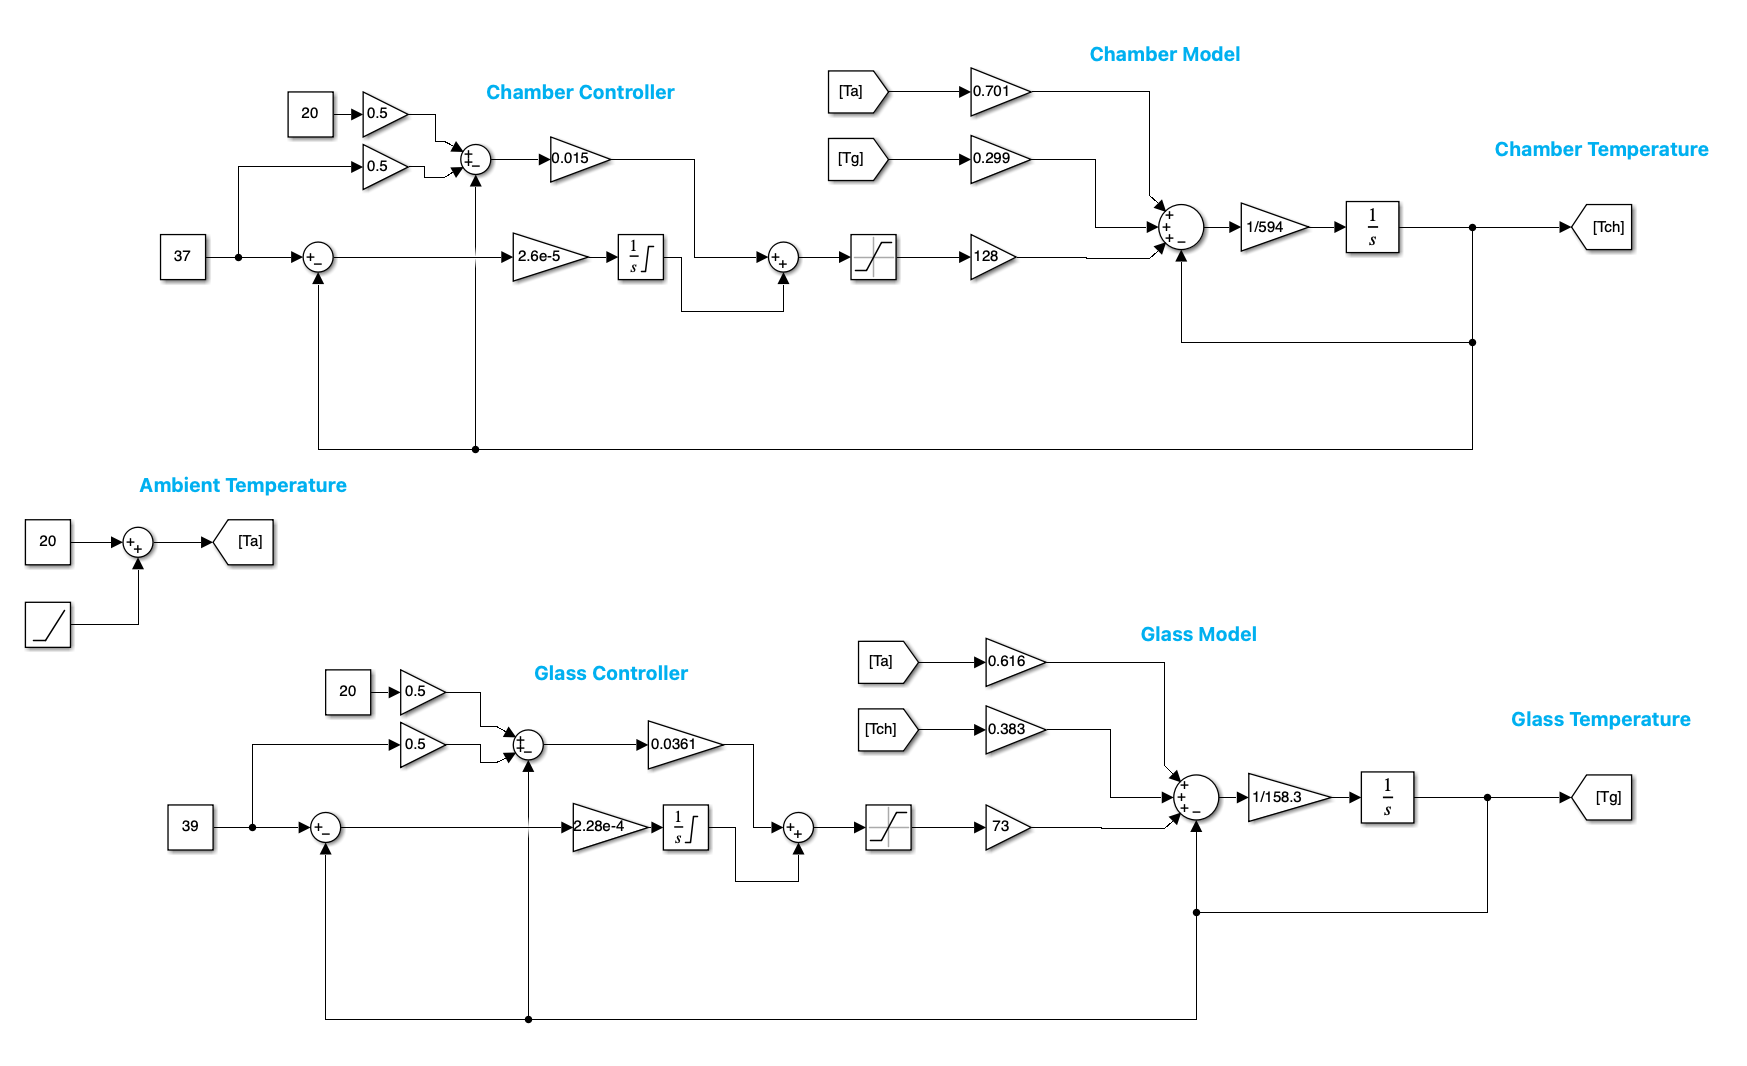
\includegraphics[width=\textwidth]{figs/Control Simulation Figures/Simulink Block Diagram Chamber and Glass.png}
    \caption[Simulink model of the coupled temperature loops]{\textbf{Simulink model of the coupled temperature loops.} Each controller uses setpoint weighting, with the room temperature recorded at start-up.}
    \label{fig_T1_simulink}
\end{figure}

\begin{figure}[htbp]
    \centering
    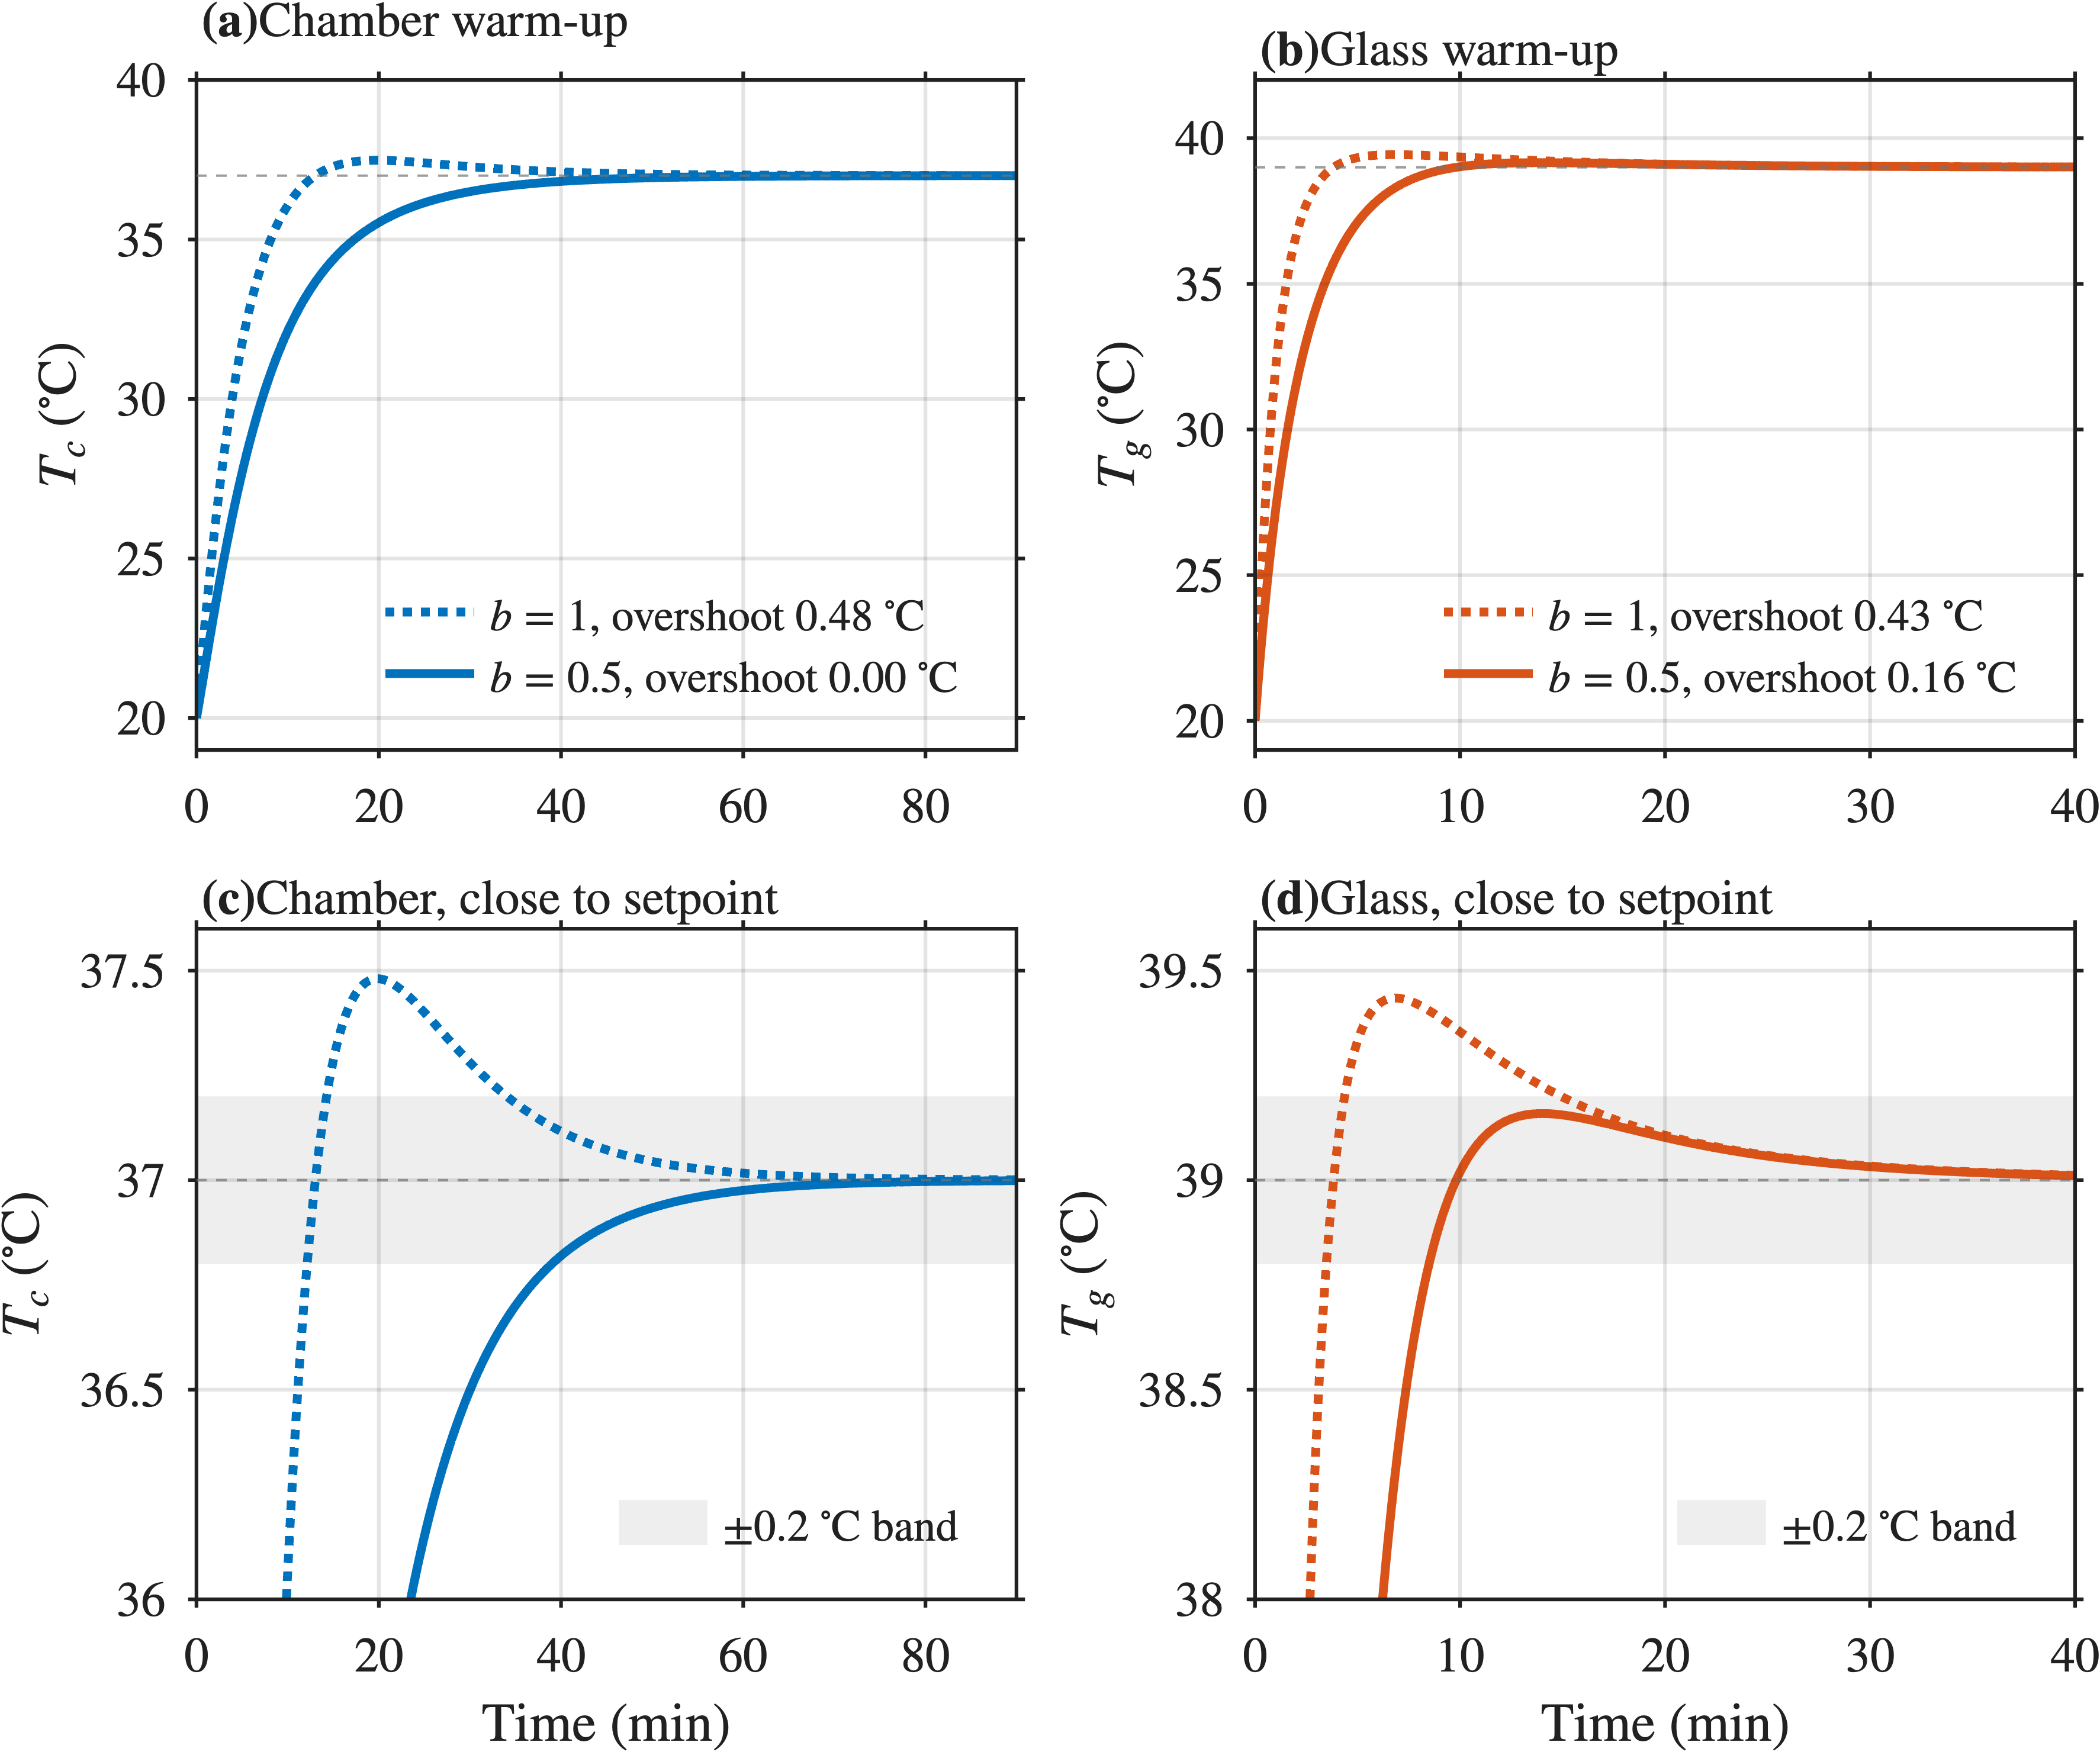
\includegraphics[width=0.74\textwidth,height=0.62\textheight,keepaspectratio]{figs/Control Simulation Figures/fig_T4_setpoint_weighting.png}
    \caption[Effect of setpoint weighting]{\textbf{Effect of setpoint weighting on warm-up,} for $b = 1$ (dotted) and $b = 0.5$ (solid). The lower panels show the approach to the setpoint with the $\pm0.2\,^\circ$C band shaded.}
    \label{fig_T4_setpoint_weighting}
\end{figure}

\begin{figure}[htbp]
    \centering
    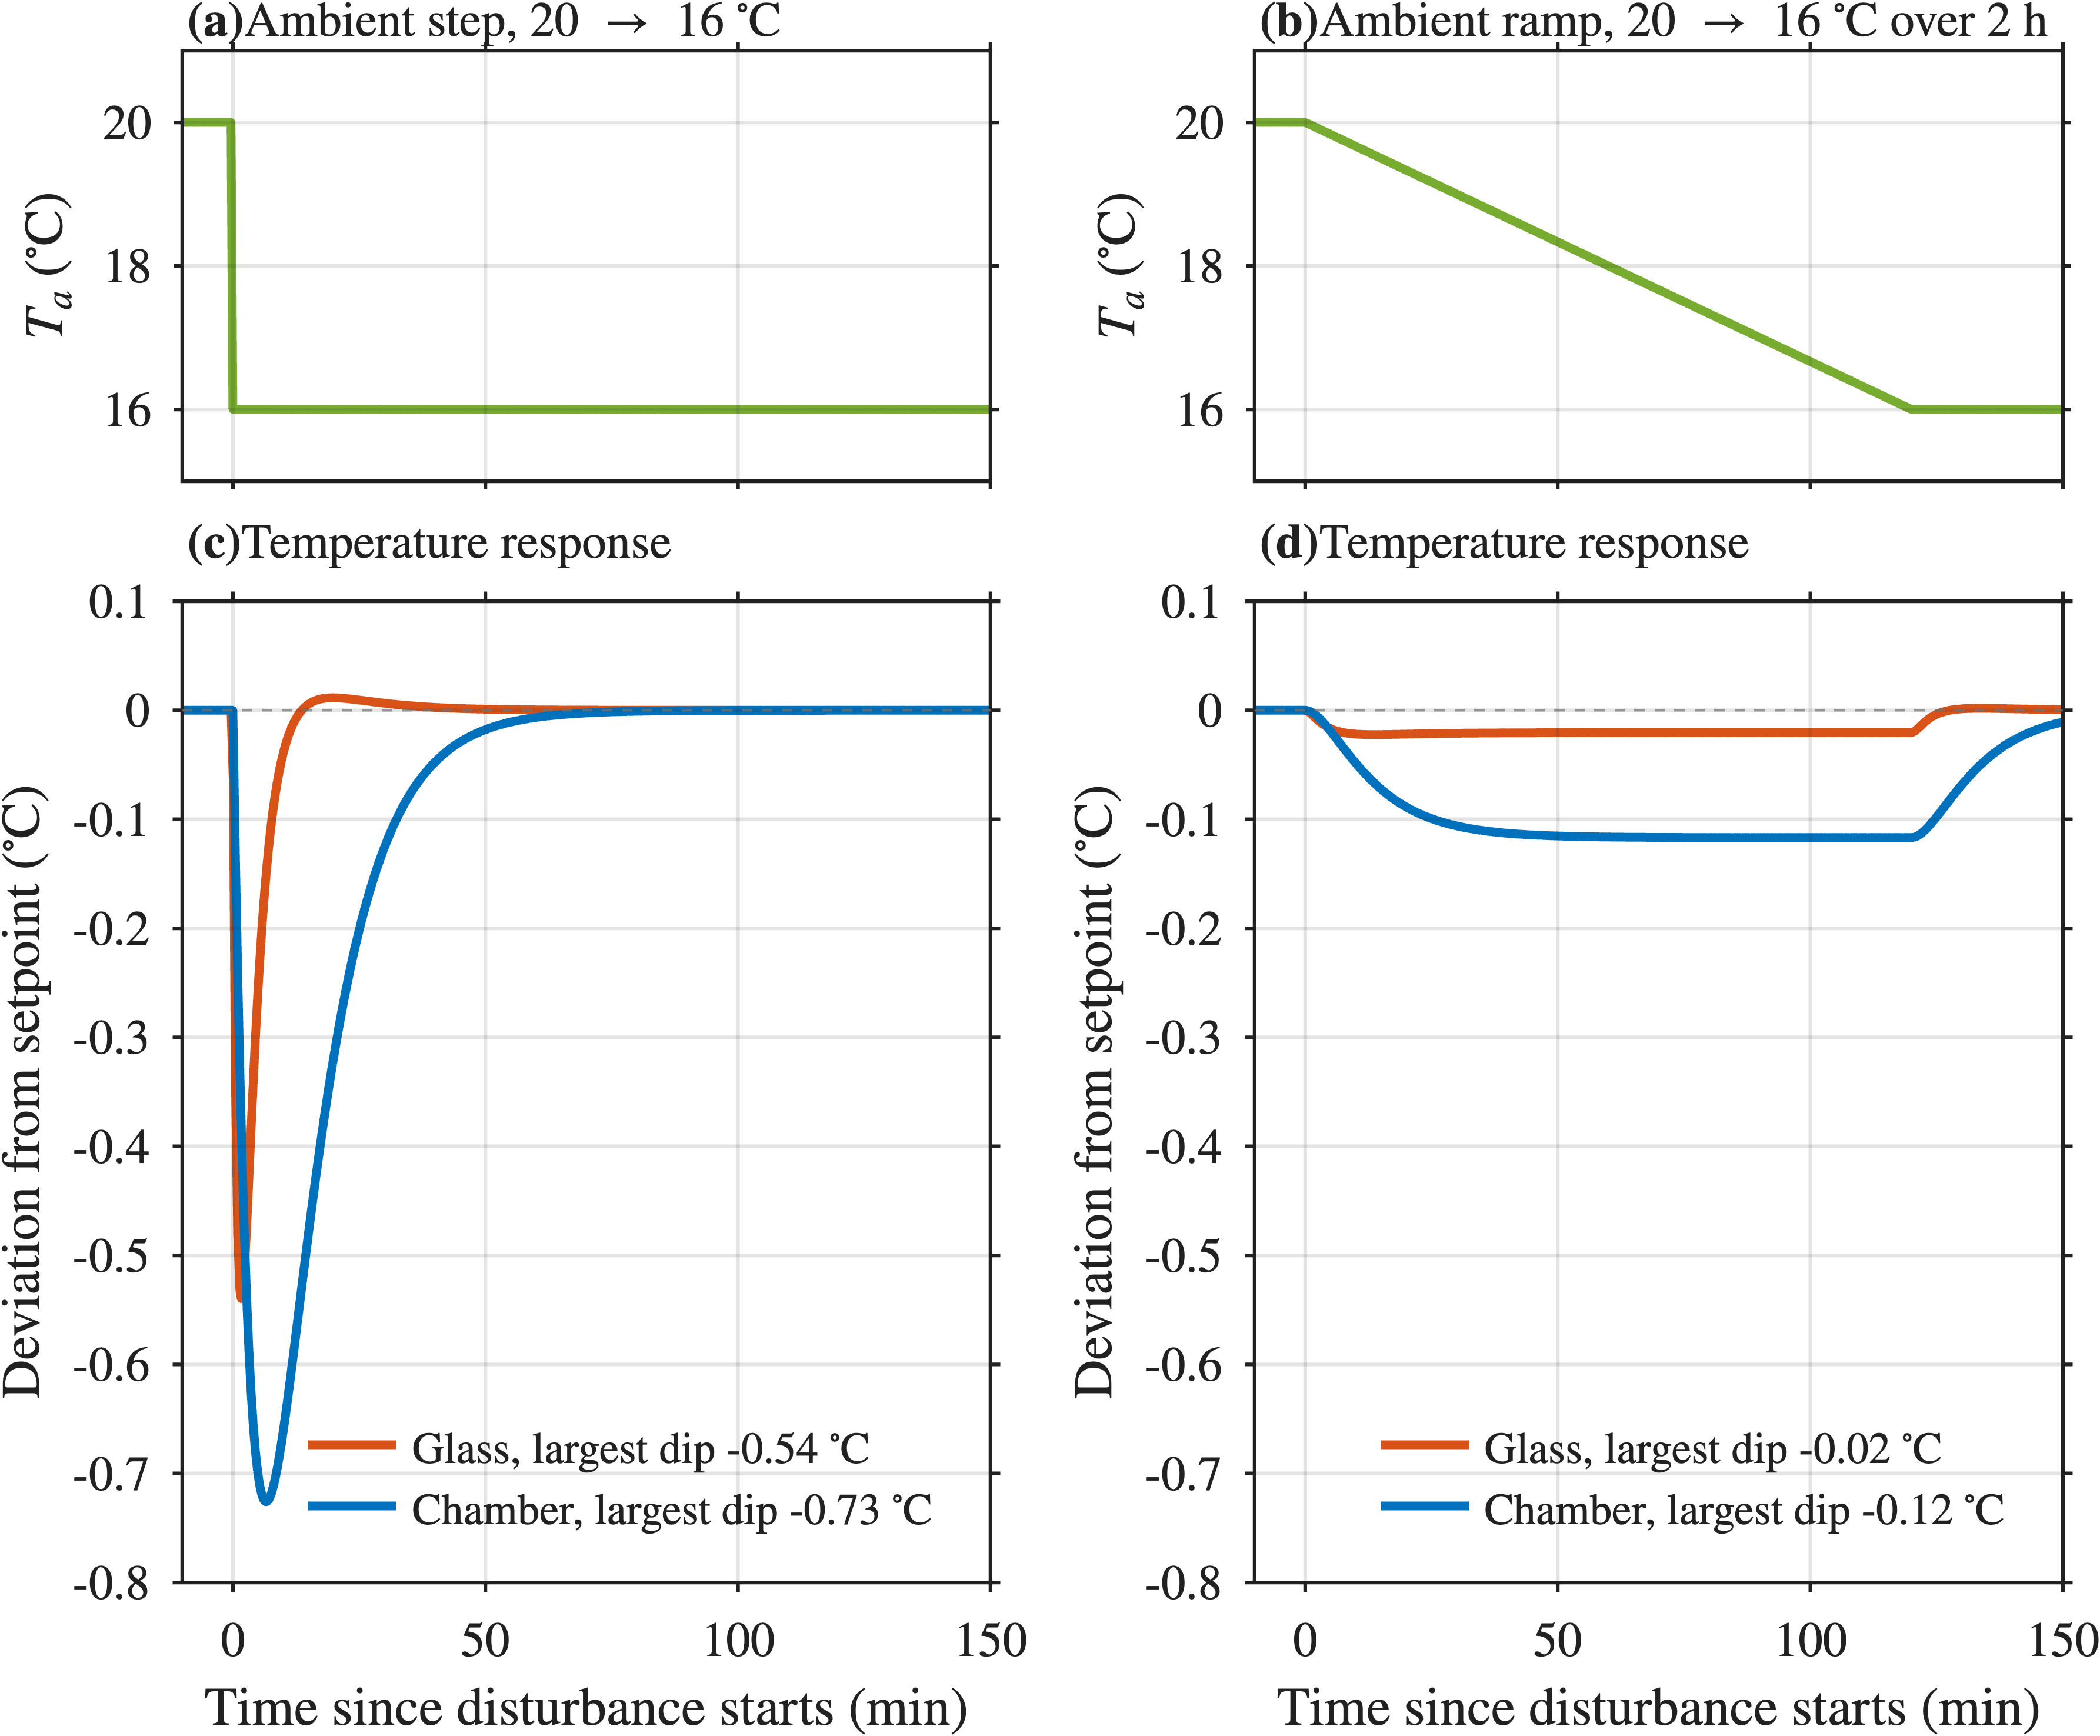
\includegraphics[width=0.74\textwidth,height=0.62\textheight,keepaspectratio]{figs/Control Simulation Figures/fig_T5_ambient_disturbances.png}
    \caption[Response to ambient temperature disturbances]{\textbf{Response to the room temperature falling from 20 to 16\,$^\circ$C,} as a step (a, c) and as a two hour ramp (b, d).}
    \label{fig_T5_ambient_disturbances}
\end{figure}

\begin{figure}[htbp]
    \centering
    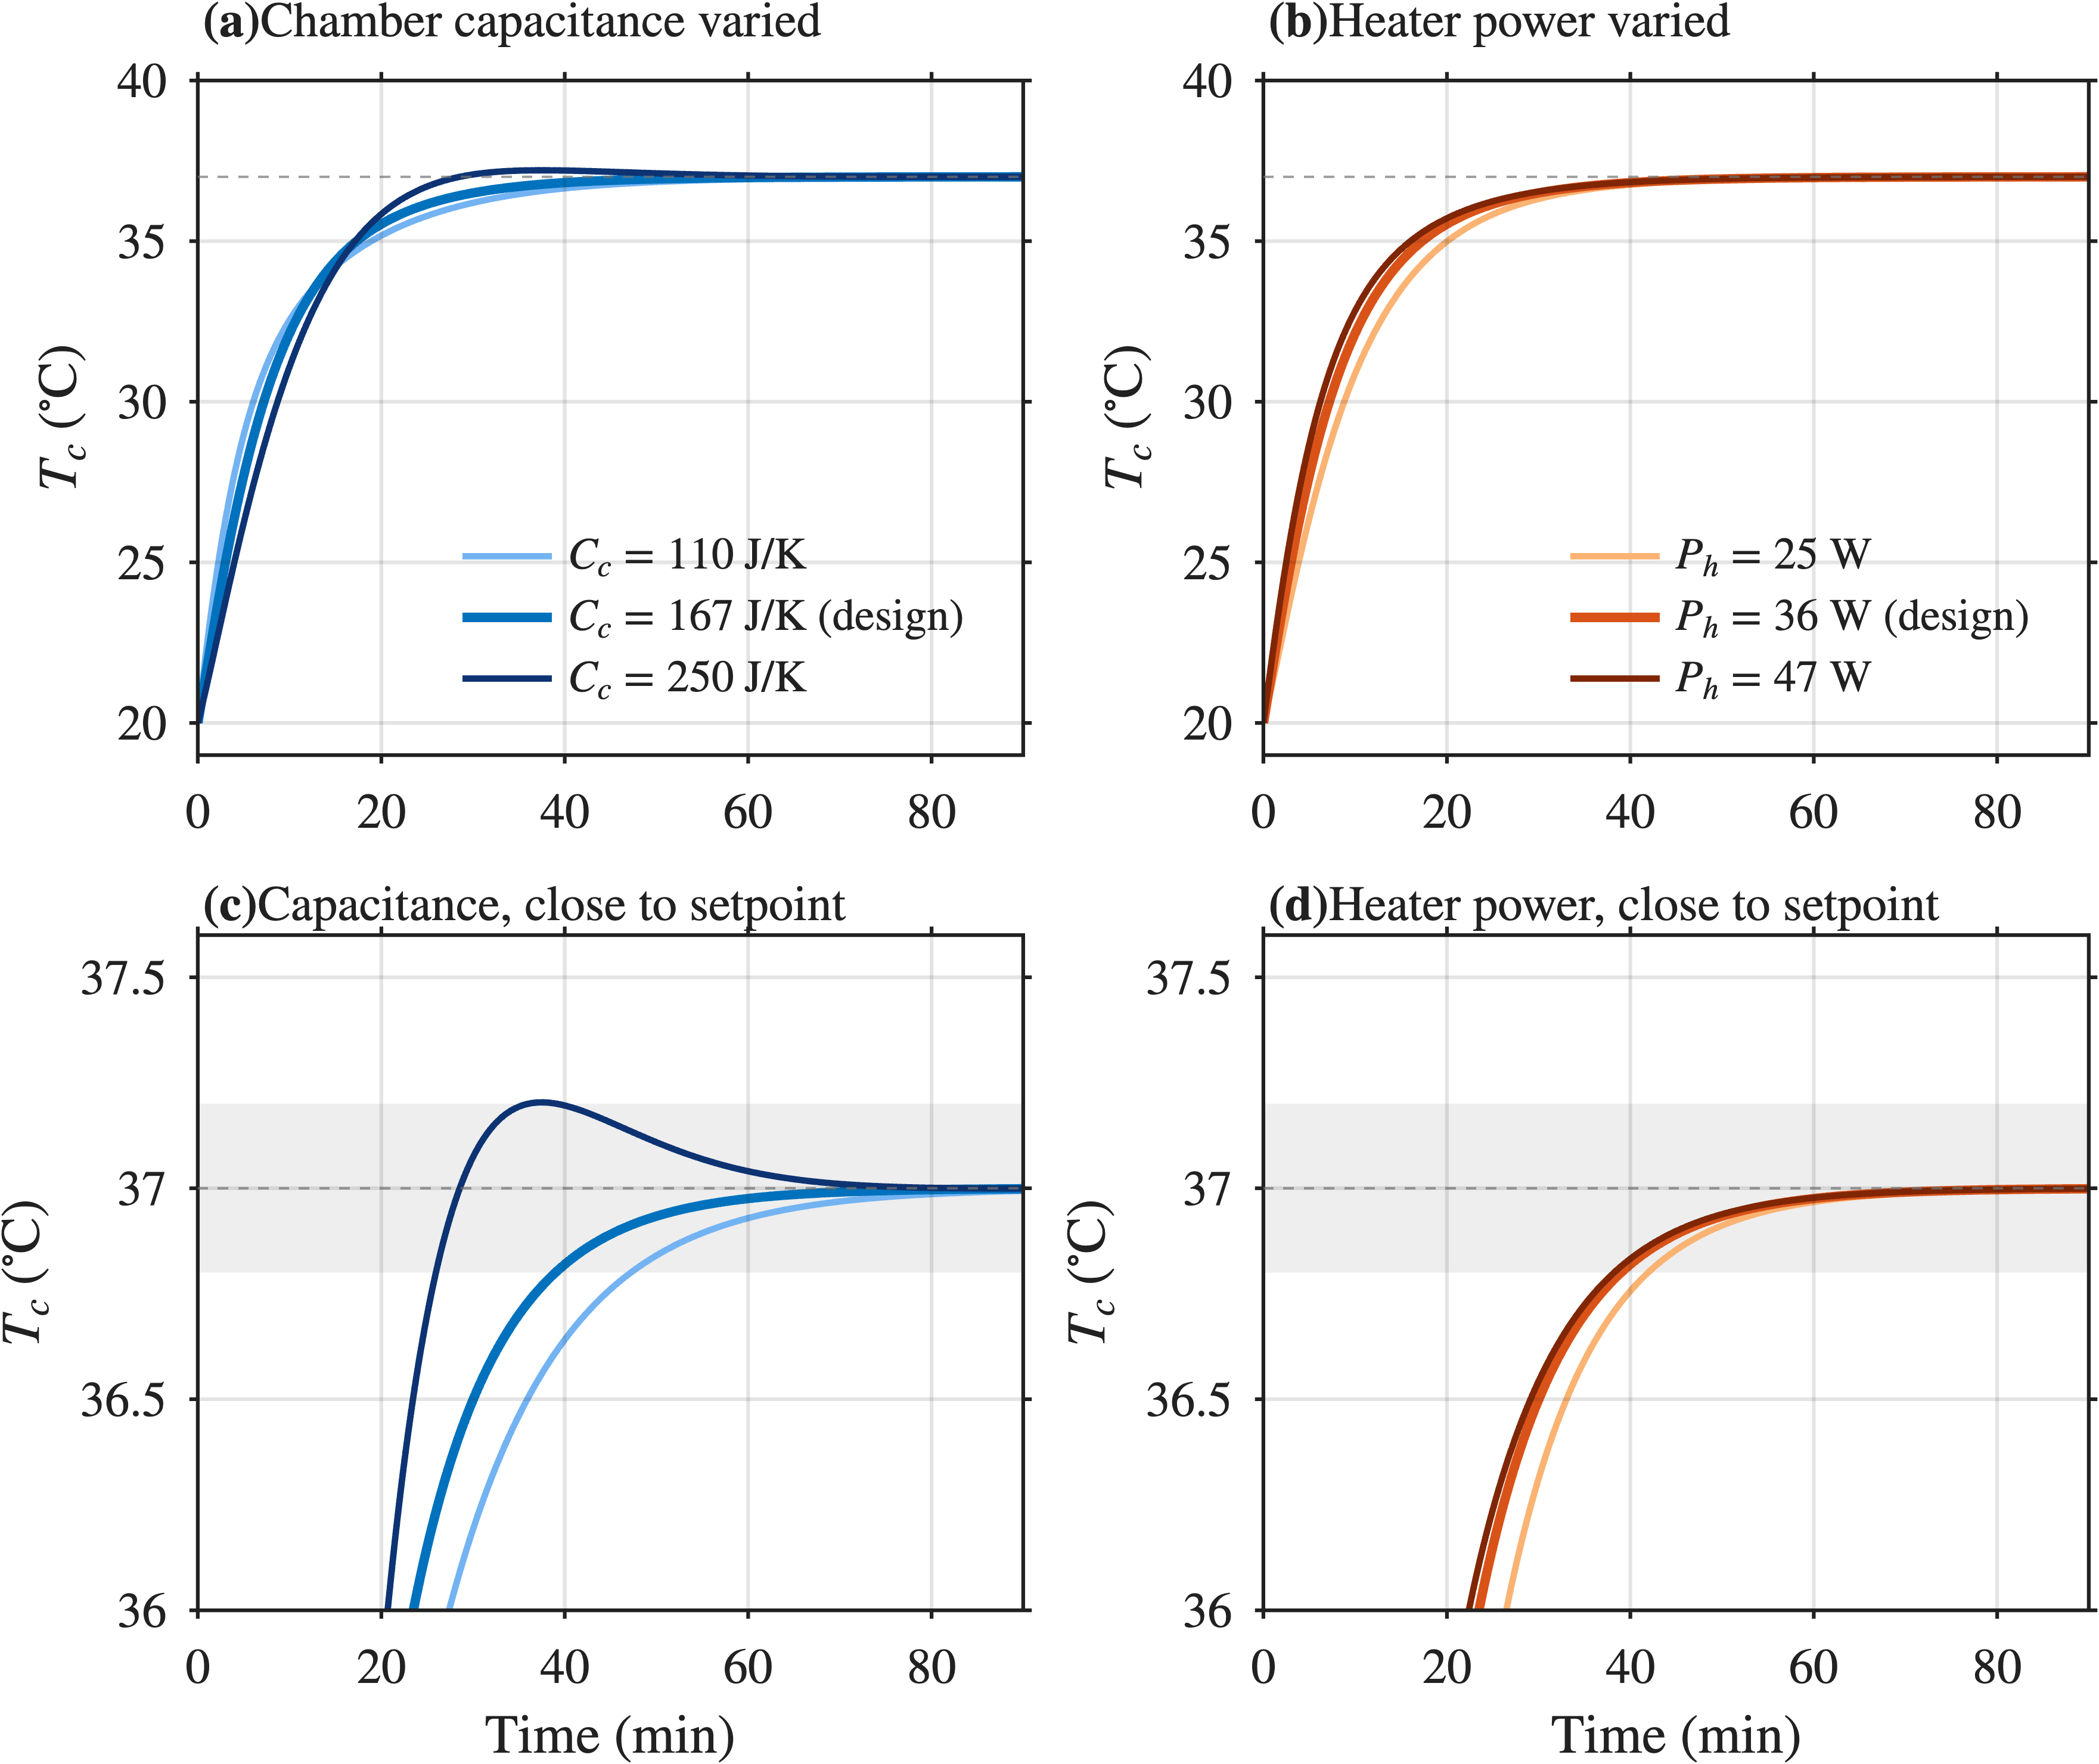
\includegraphics[width=0.74\textwidth,height=0.62\textheight,keepaspectratio]{figs/Control Simulation Figures/fig_T6_robustness.png}
    \caption[Robustness of the chamber loop to model error]{\textbf{Robustness of the chamber loop to model error.} The controller is tuned for $C_c = 167$\,J/K and $P_h = 36$\,W, and the simulated plant uses the values shown.}
    \label{fig_T6_robustness}
\end{figure}

\begin{figure}[htbp]
    \centering
    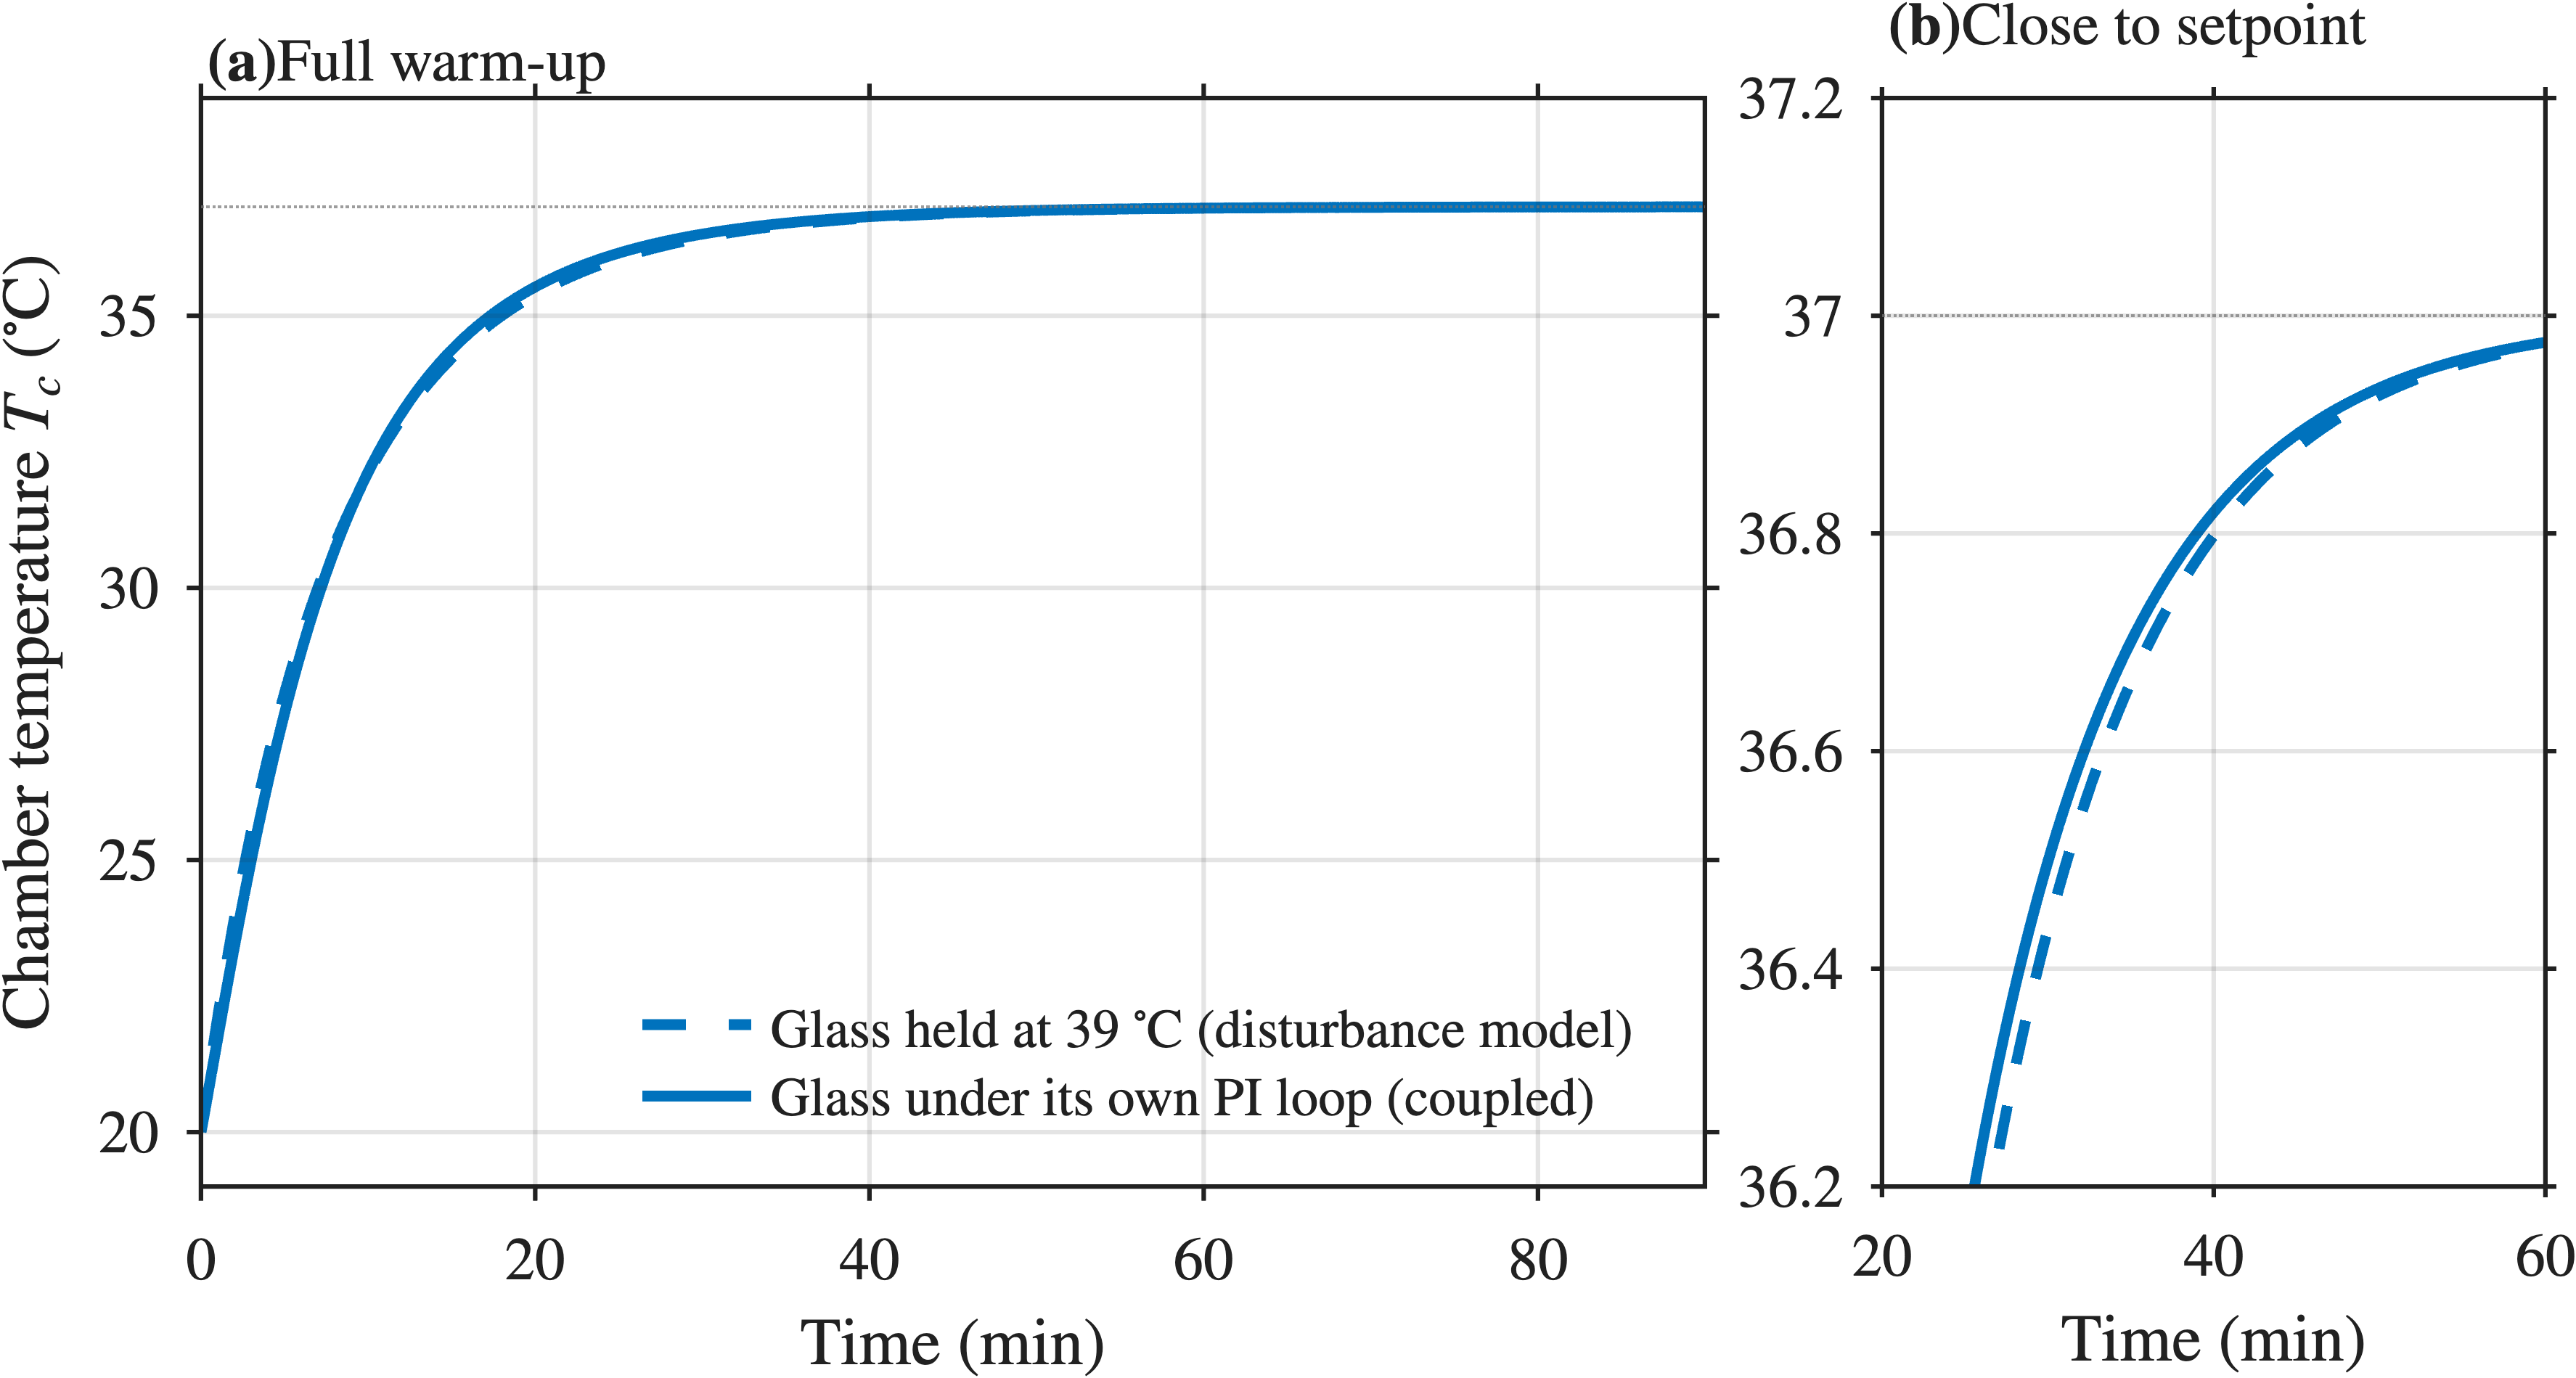
\includegraphics[width=0.74\textwidth,height=0.62\textheight,keepaspectratio]{figs/Control Simulation Figures/fig_T7_glass_fixed_vs_coupled.png}
    \caption[Chamber warm-up with a fixed and a controlled glass]{\textbf{Chamber warm-up with the glass held at 39\,$^\circ$C and with the glass under its own loop.} The two curves nearly overlap, so the loops can be designed separately.}
    \label{fig_T7_glass_fixed_vs_coupled}
\end{figure}

\begin{figure}[htbp]
    \centering
    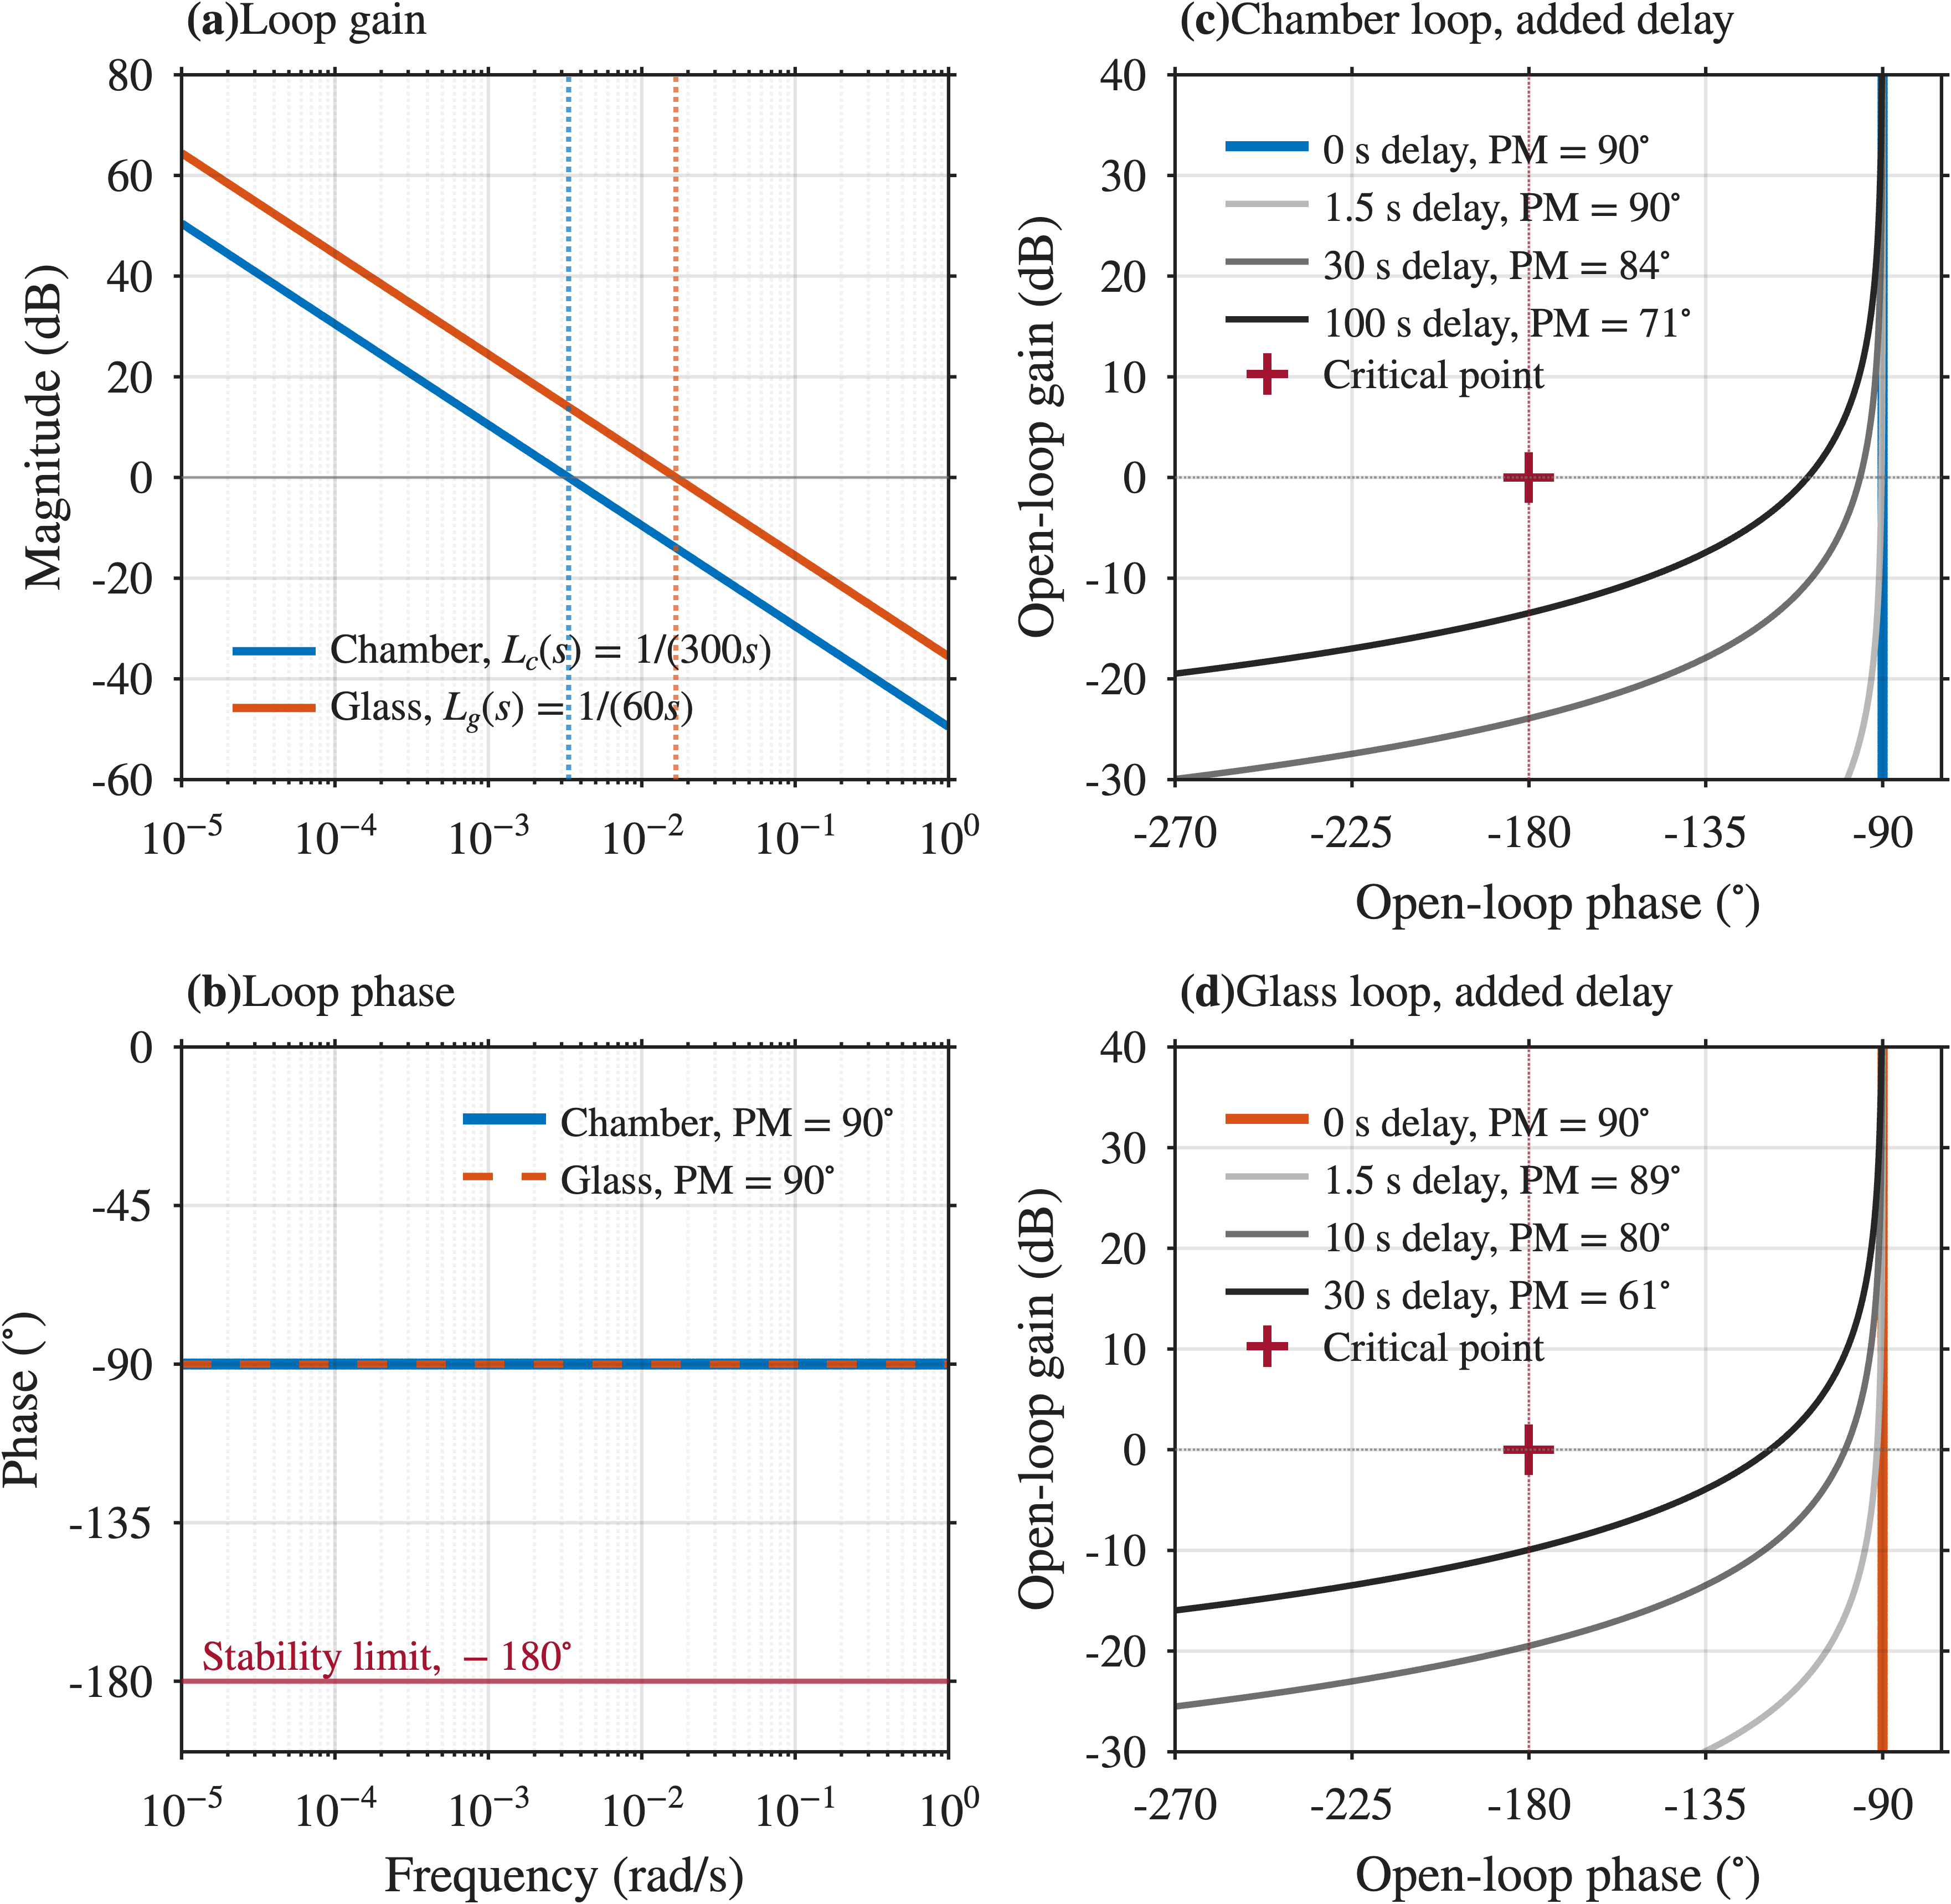
\includegraphics[width=0.74\textwidth,height=0.62\textheight,keepaspectratio]{figs/Control Simulation Figures/fig_T8_bode_nichols.png}
    \caption[Open-loop frequency response of the temperature loops]{\textbf{Open-loop frequency response of the temperature loops.} (a, b) Bode plots. (c, d) Nichols charts with added delay and the resulting phase margins.}
    \label{fig_T8_bode_nichols}
\end{figure}

\begin{figure}[htbp]
    \centering
    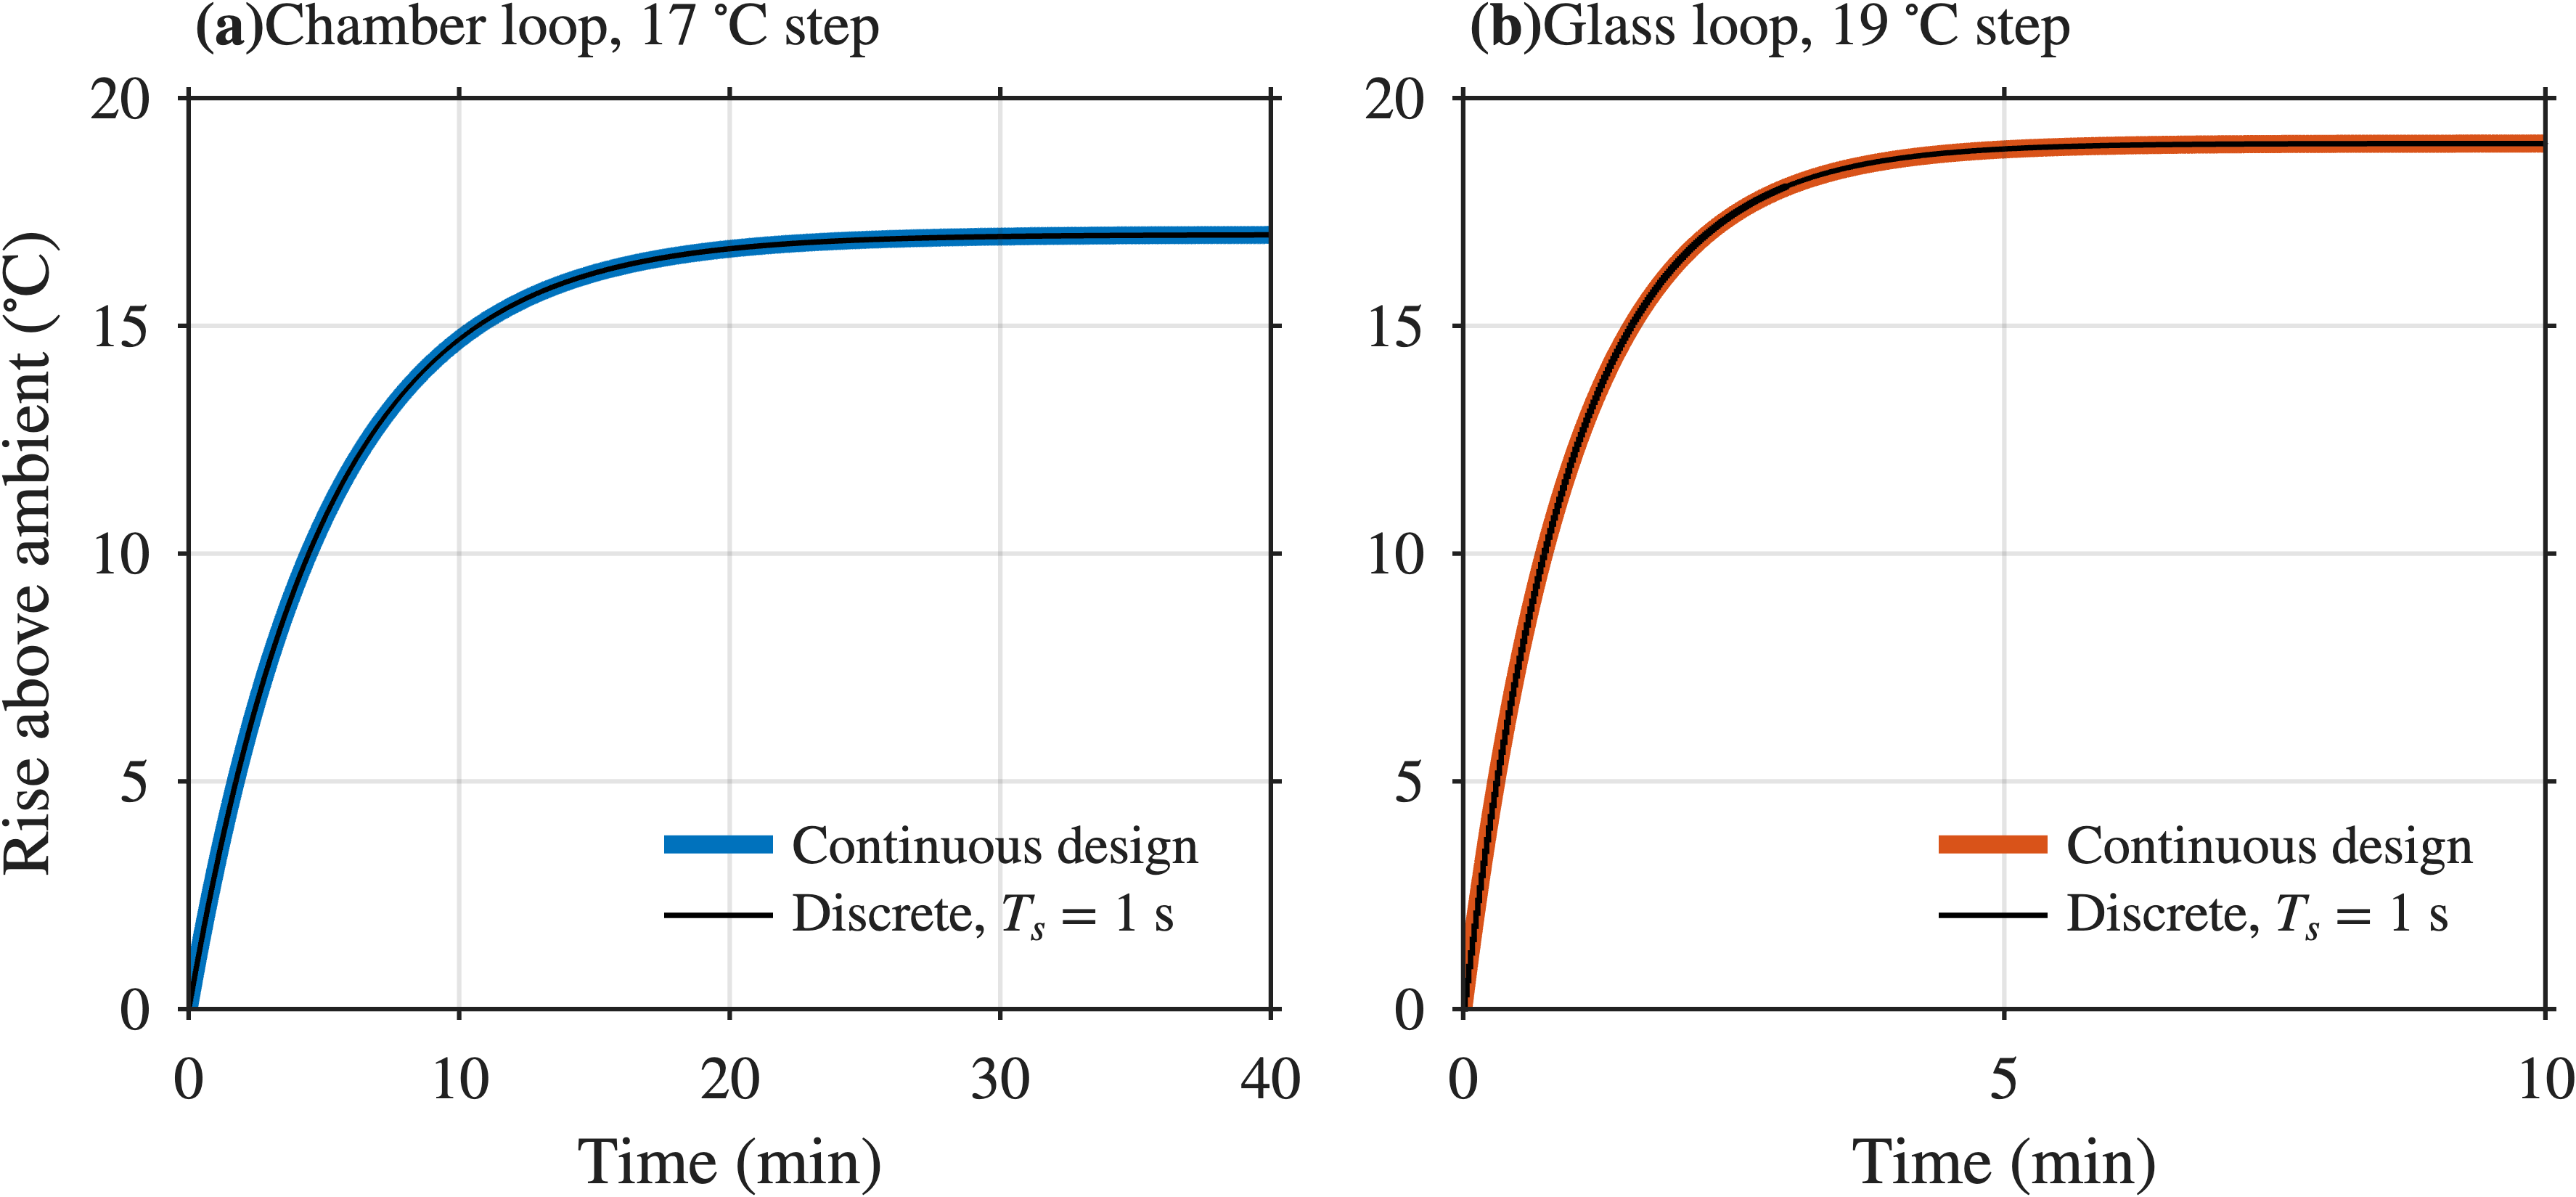
\includegraphics[width=0.74\textwidth,height=0.62\textheight,keepaspectratio]{figs/Control Simulation Figures/fig_T9_discrete_vs_continuous.png}
    \caption[Continuous design against digital implementation]{\textbf{Continuous design against the digital implementation} with a 1\,s sample time.}
    \label{fig_T9_discrete_vs_continuous}
\end{figure}

\FloatBarrier
\section{CO\textsubscript{2} Control}
\label{app:co2-control-sim}

This section supports Section~\ref{subsec:co2-control} and uses the design volume of 0.99\,L. Figure~\ref{fig_C1_simulink} shows the Simulink model of the loop. Figures~\ref{fig_C3_fill_strategies} and~\ref{fig_C4_lid_openings} compare two ways of filling the chamber and show the recovery after the lid is opened. Figure~\ref{fig_C5_robustness} varies the leak and the flow, Figure~\ref{fig_C6_valve_pulses} shows the valve pulses at steady state, and Figure~\ref{fig_C7_bode} gives the frequency response. These results were repeated for the built chamber volume of 0.47\,L in Appendix~\ref{app:co2-humidity}, and those results replace these ones where they differ.

\begin{figure}[htbp]
    \centering
    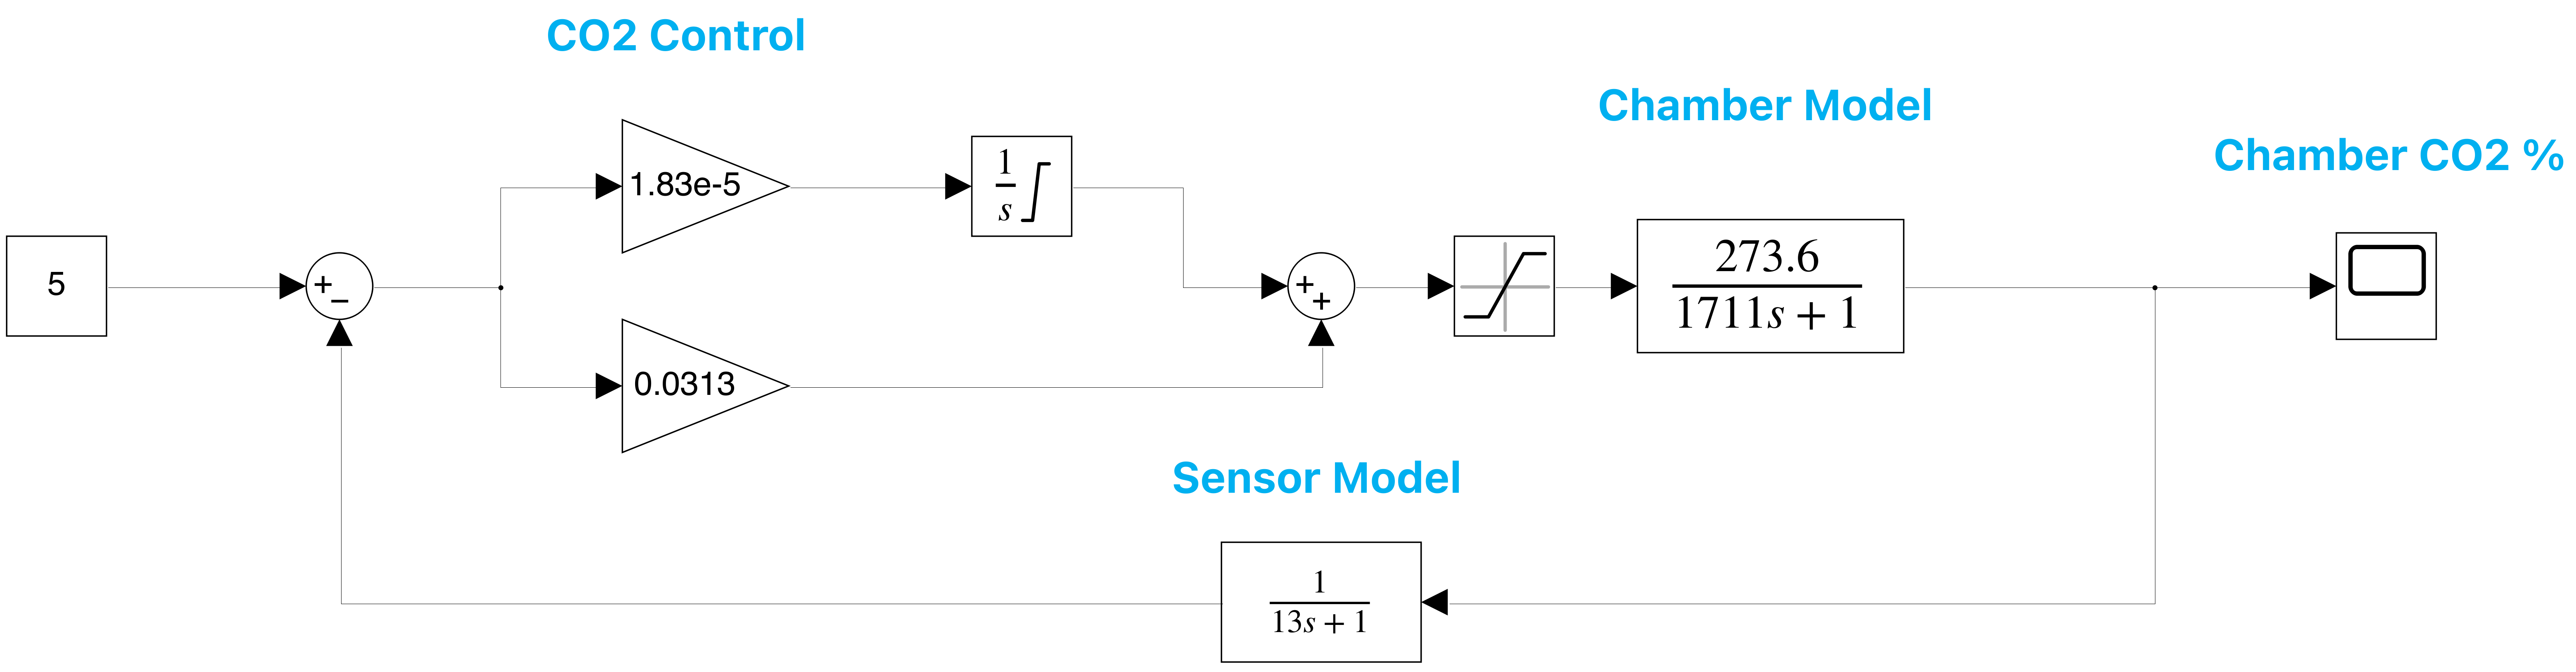
\includegraphics[width=\textwidth]{figs/Control Simulation Figures/fig_C1_simulink.png}
    \caption[Simulink model of the CO\textsubscript{2} loop]{\textbf{Simulink model of the CO\textsubscript{2} loop,} using the linearised chamber model and a first order sensor lag.}
    \label{fig_C1_simulink}
\end{figure}

\begin{figure}[htbp]
    \centering
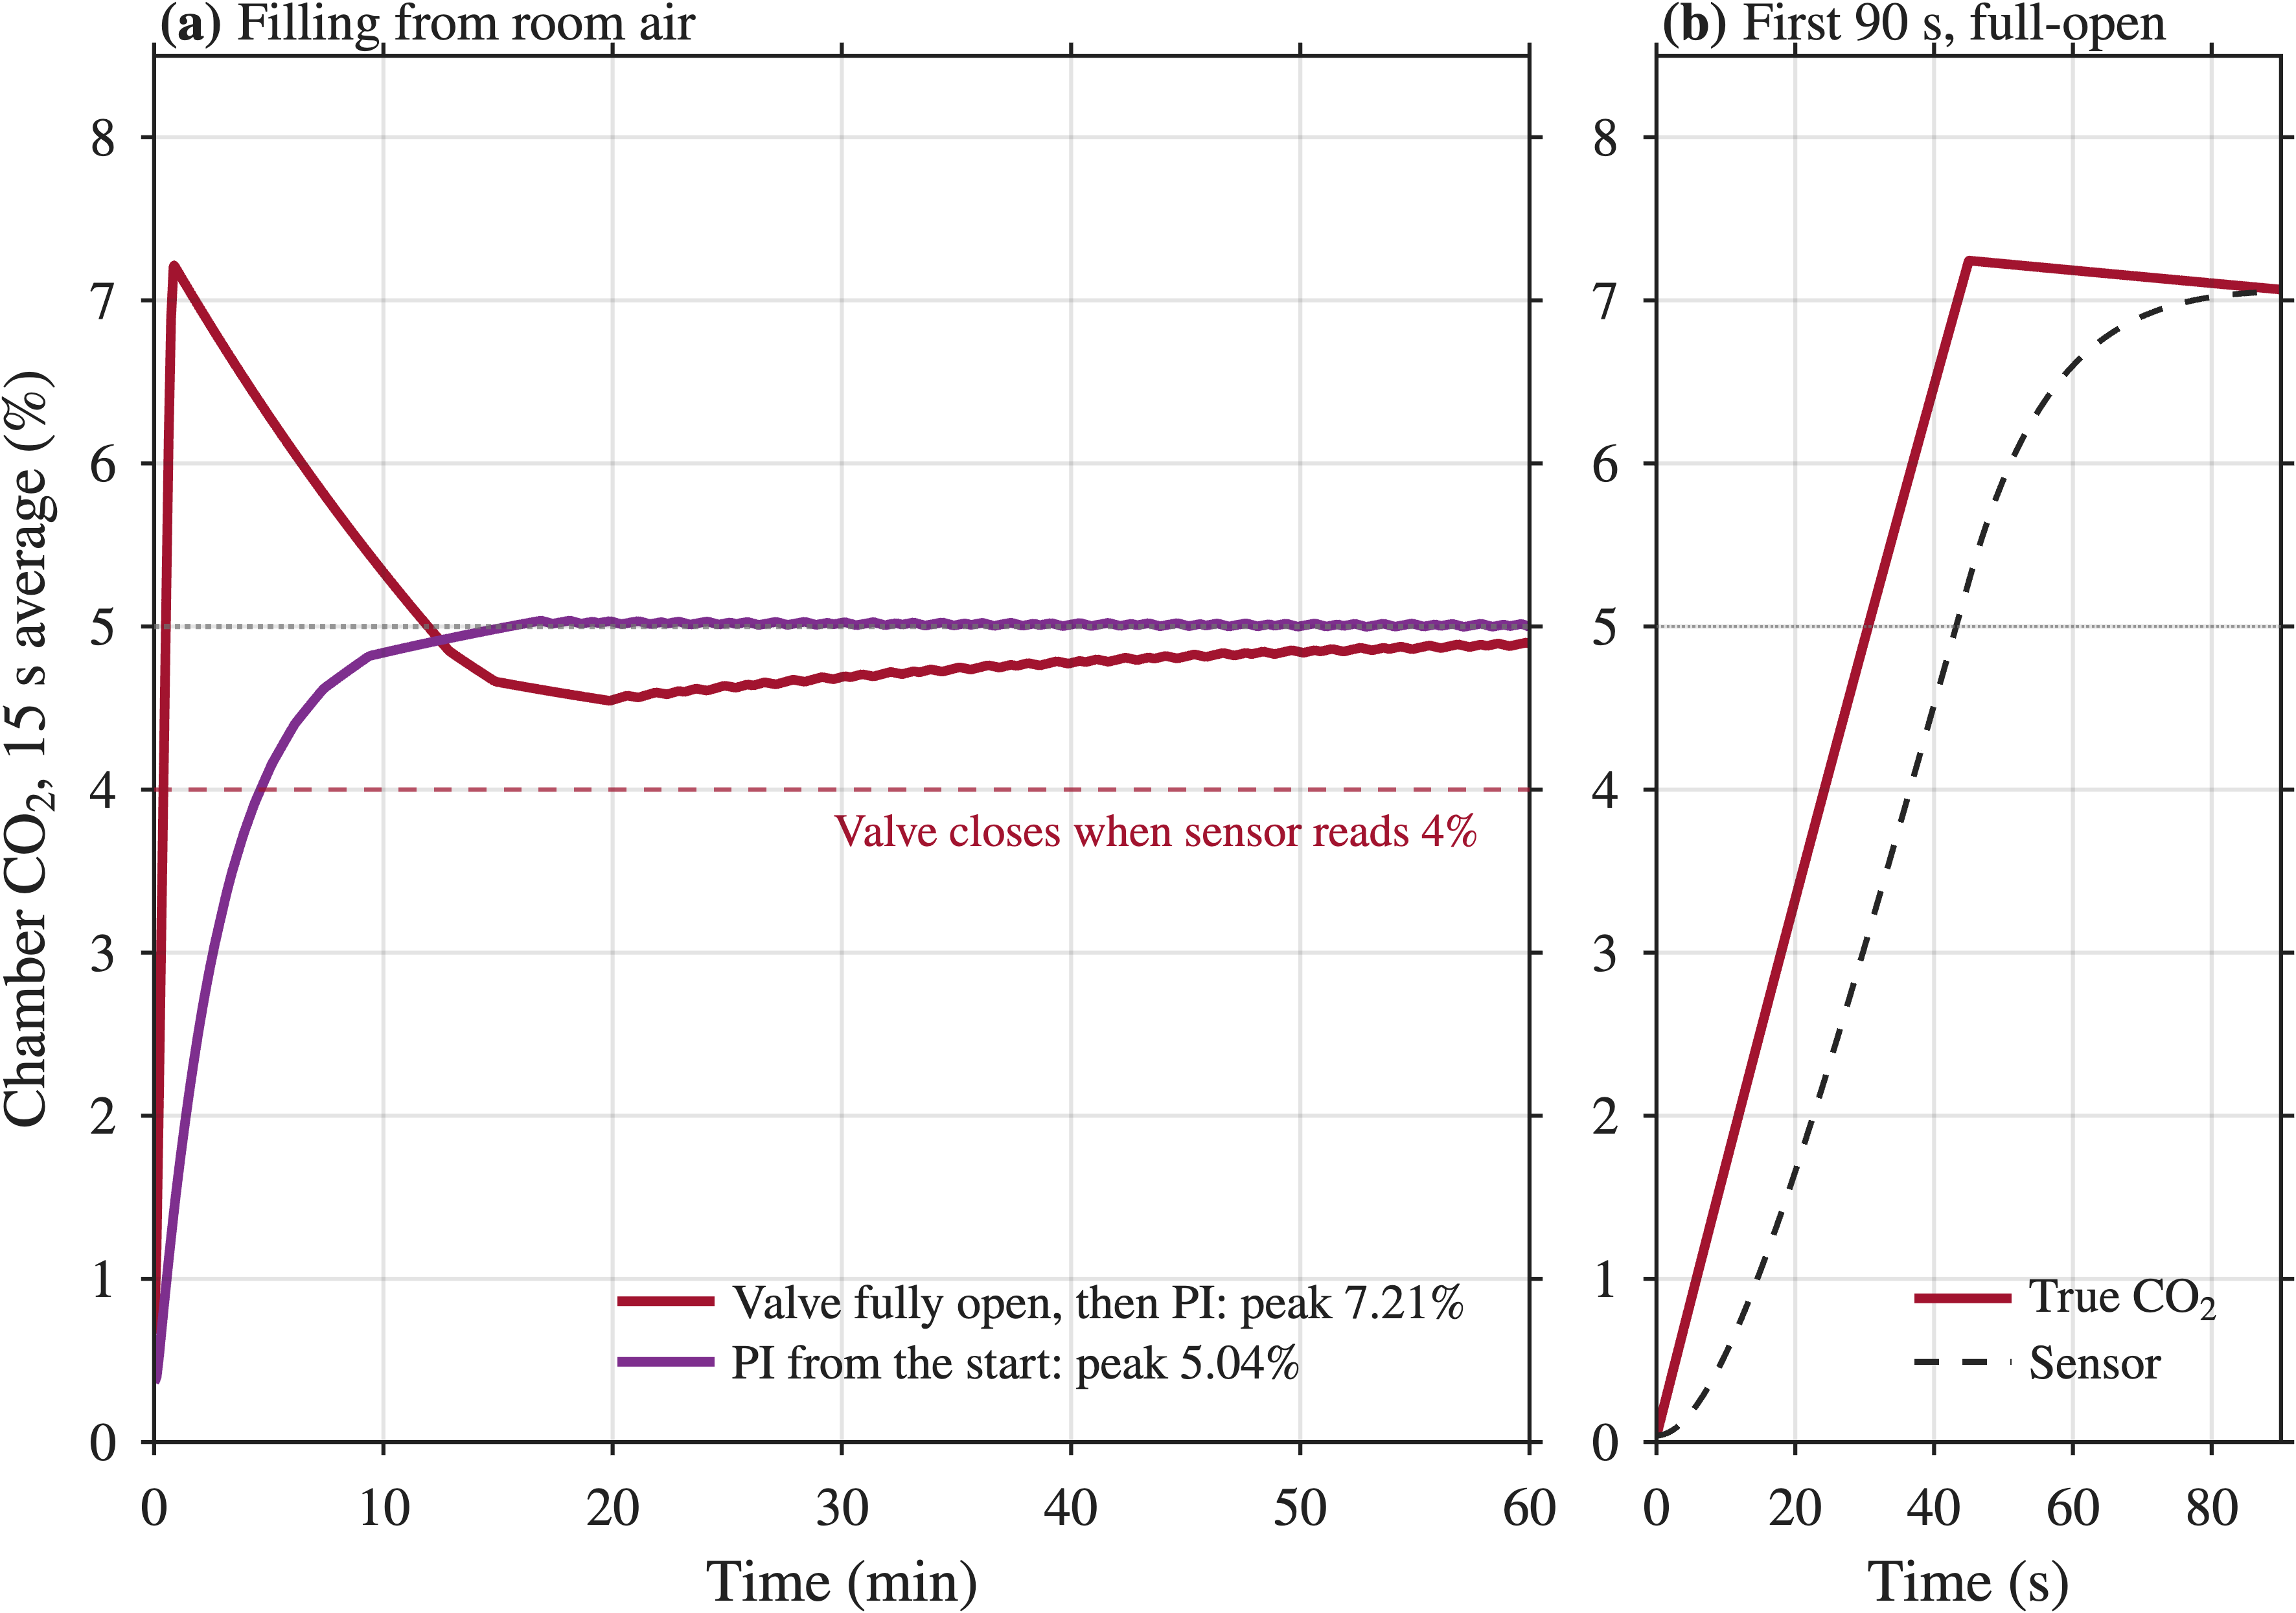
\includegraphics[width=0.74\textwidth,height=0.62\textheight,keepaspectratio]{figs/Control Simulation Figures/fig_C3_fill_strategies.png}
    \caption[Comparison of fill strategies]{\textbf{PI fill against holding the valve open until the sensor reads 4\%.} (b) The first 90\,s, where the sensor lags the actual concentration.}
    \label{fig_C3_fill_strategies}
\end{figure}

\begin{figure}[htbp]
    \centering
    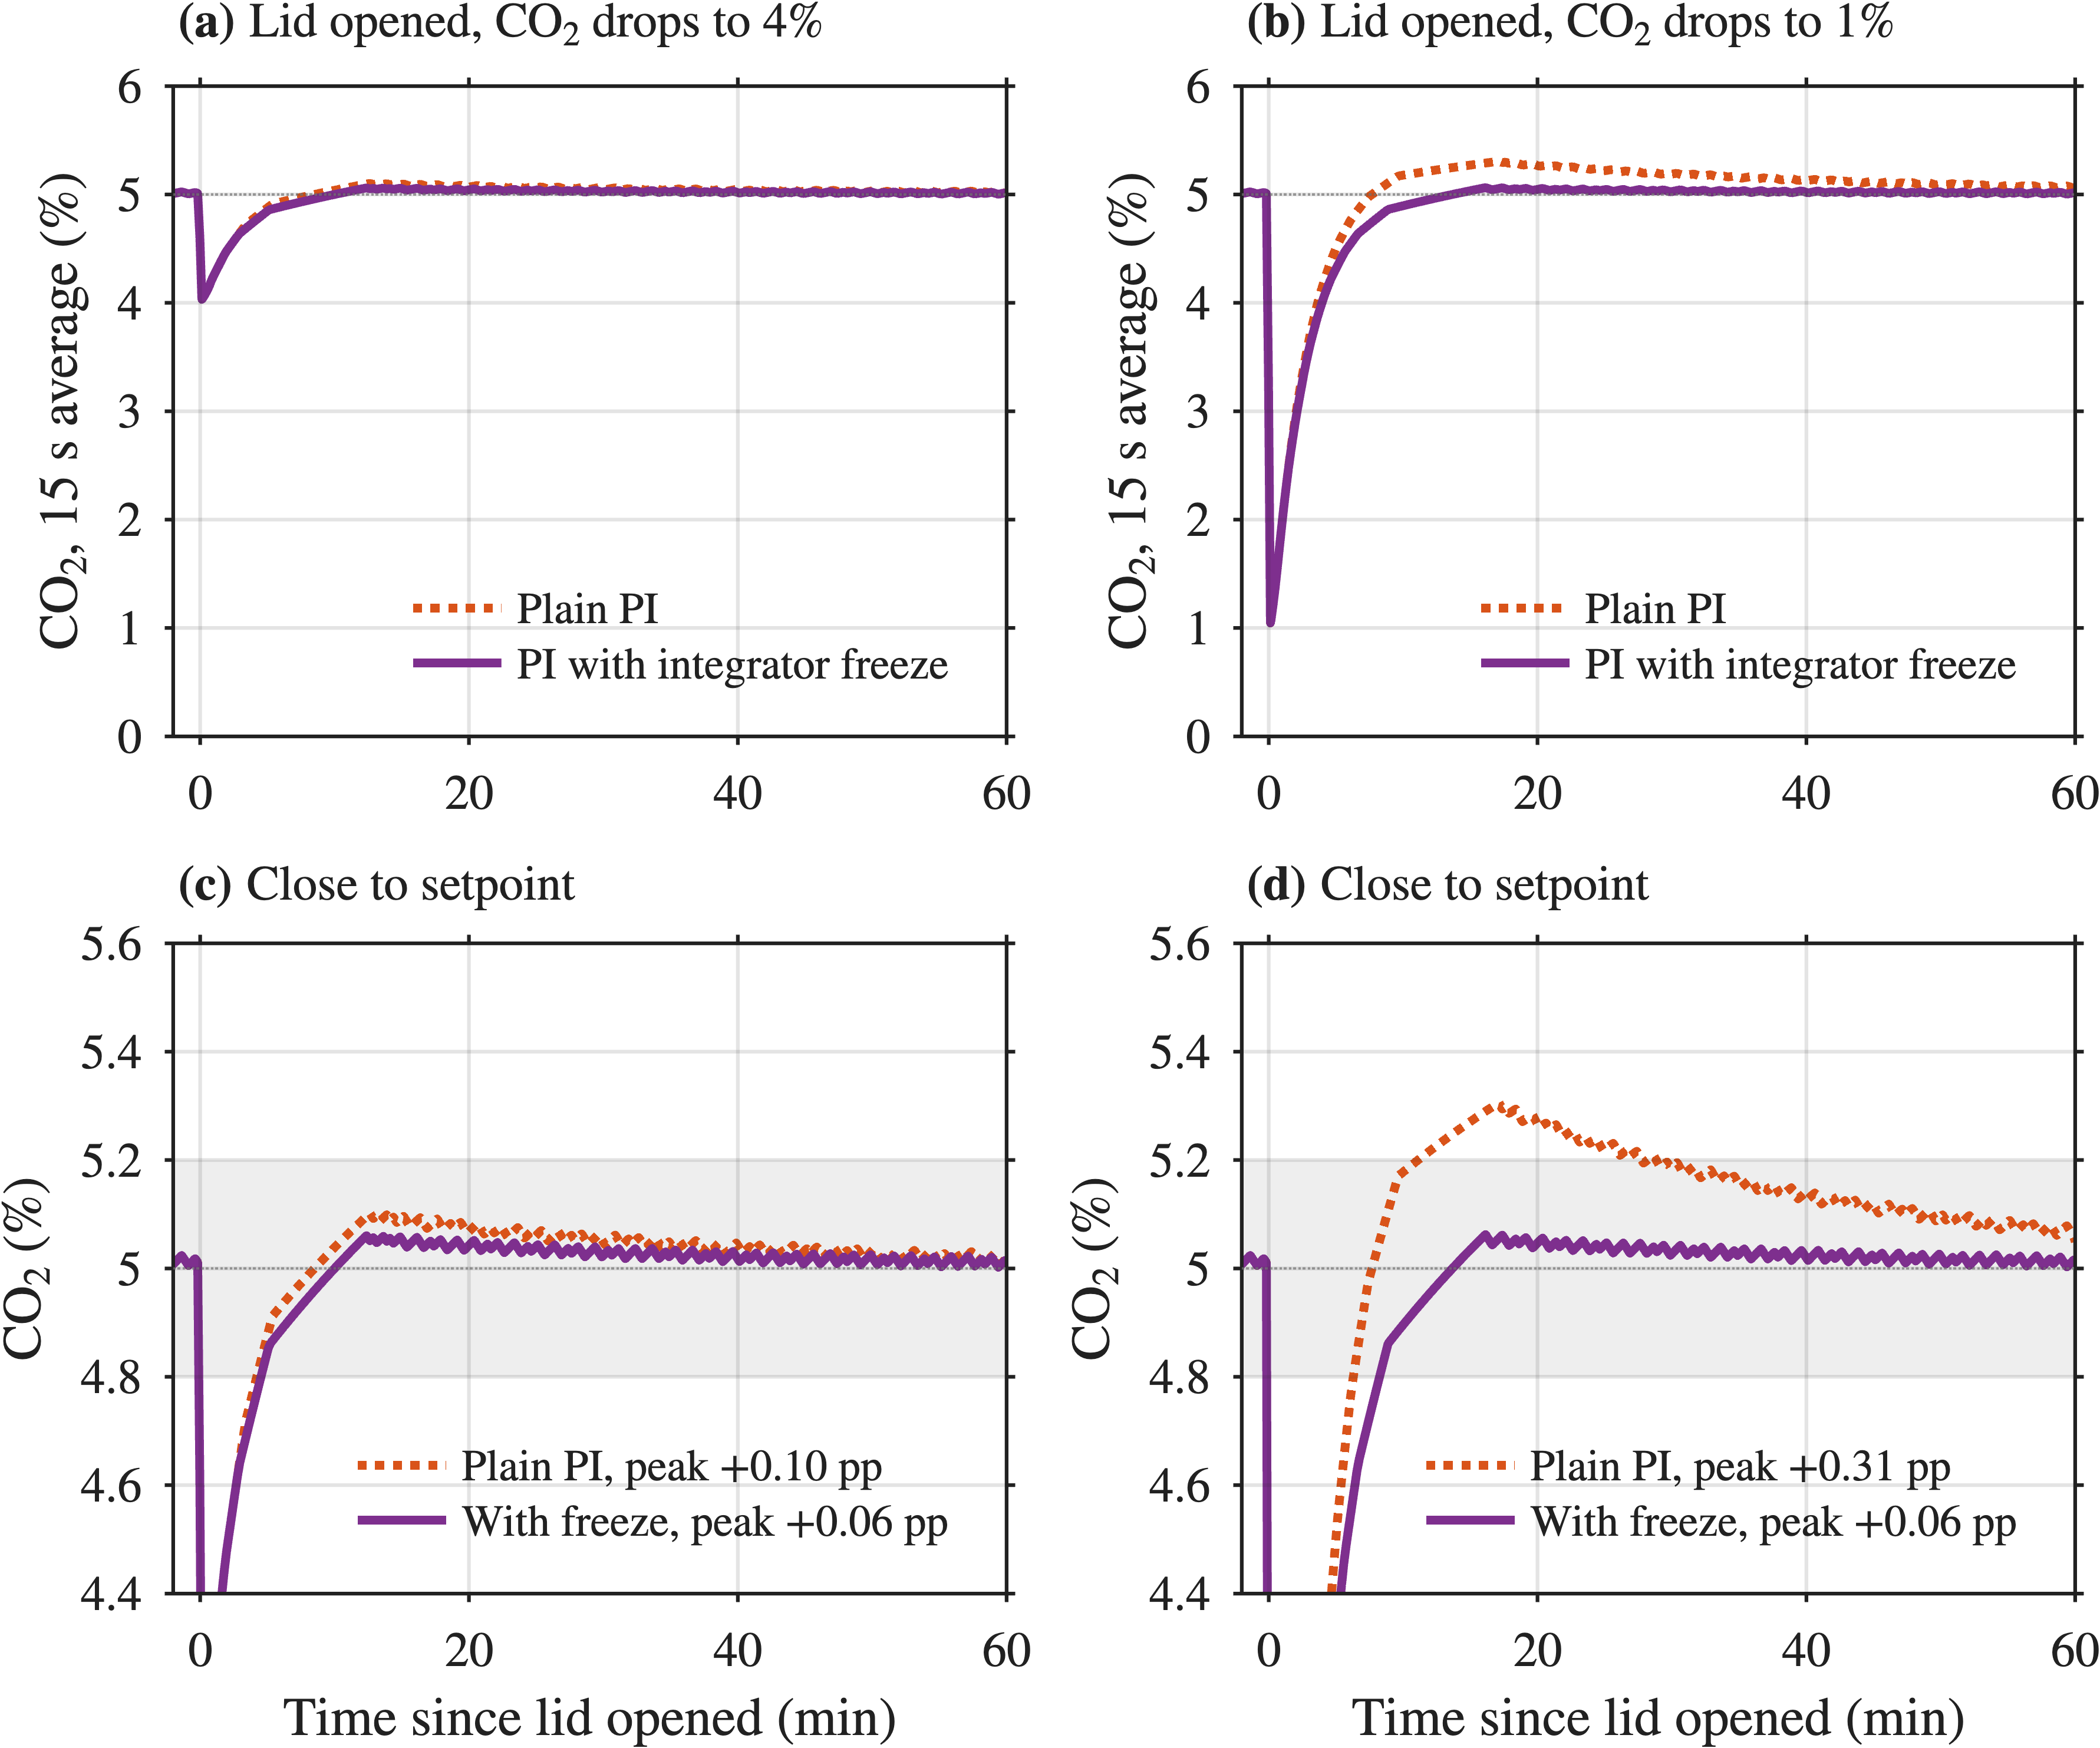
\includegraphics[width=0.6\textwidth]{figs/Control Simulation Figures/fig_C4_lid_openings.png}
    \caption[Recovery after lid openings]{\textbf{Recovery after lid openings,} with the plain PI and with the integrator freeze. (c, d) show the approach to the setpoint.}
    \label{fig_C4_lid_openings}
\end{figure}

\begin{figure}[htbp]
    \centering
    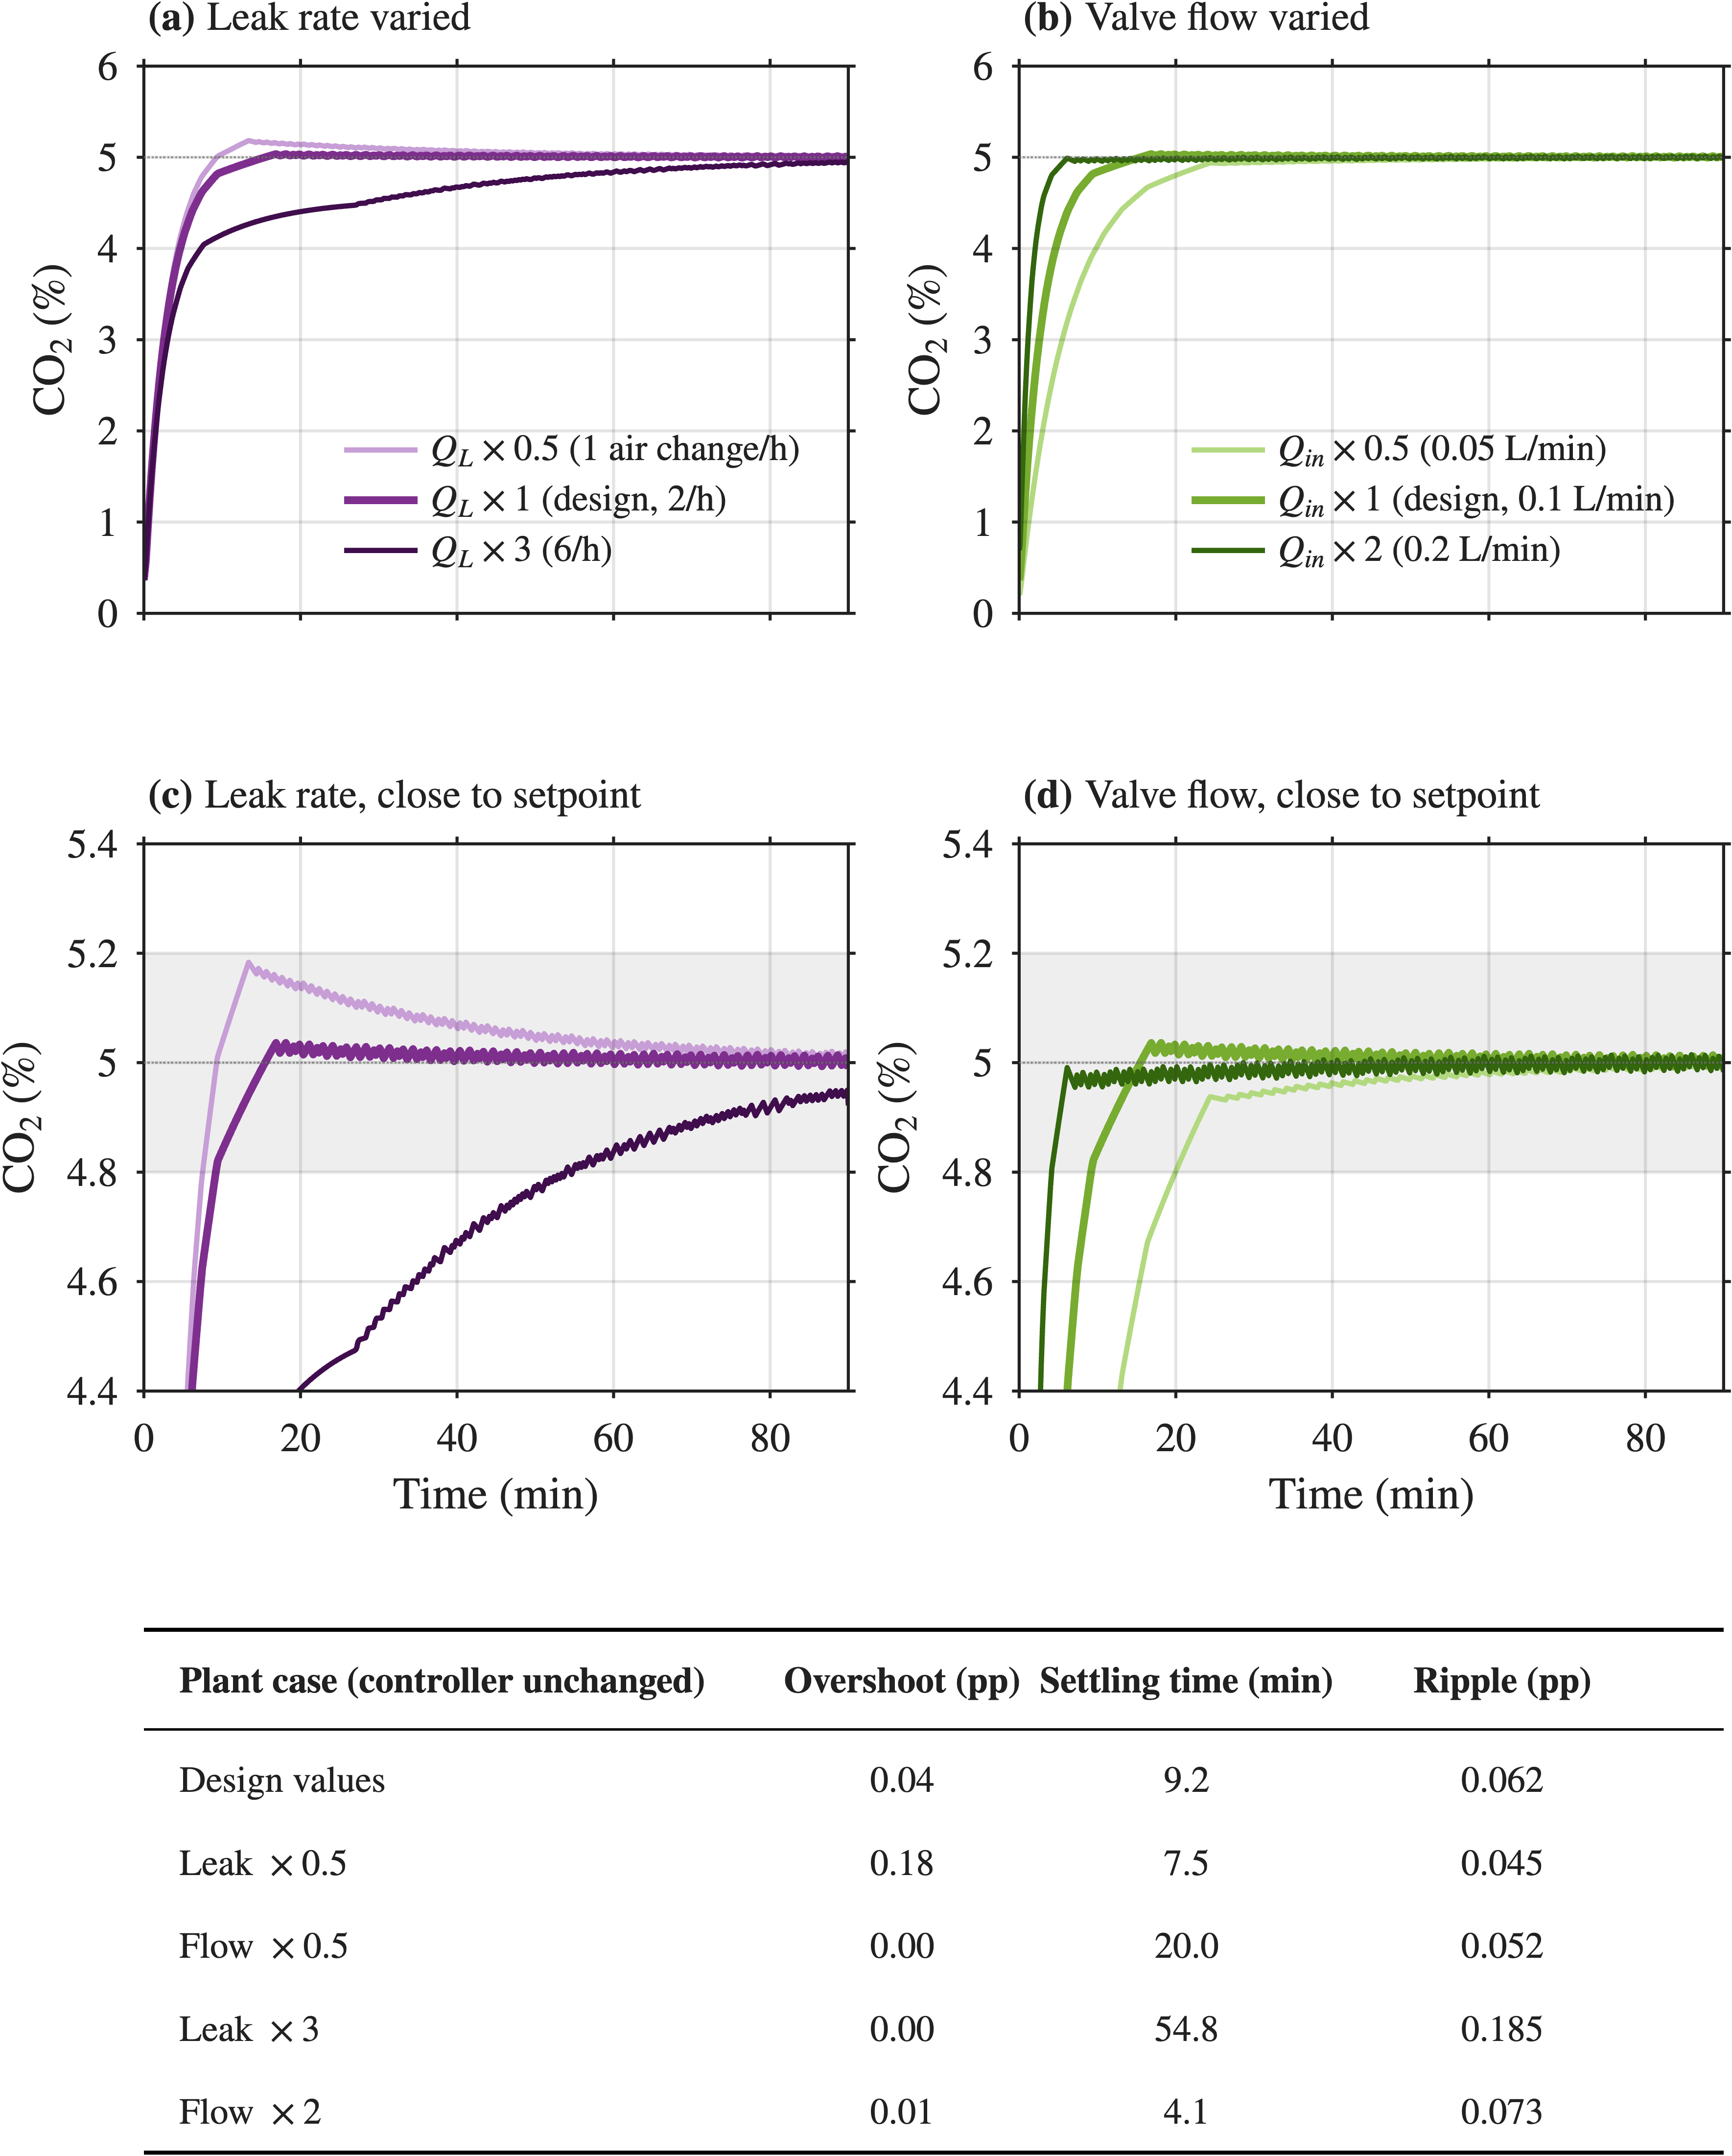
\includegraphics[width=0.6\textwidth]{figs/Control Simulation Figures/fig_C5_robustness.png}
    \caption[Robustness of the CO\textsubscript{2} loop]{\textbf{Robustness of the CO\textsubscript{2} loop to the leak rate and valve flow.} The controller is tuned for the design values, and the simulated plant uses the values shown.}
    \label{fig_C5_robustness}
\end{figure}

\begin{figure}[htbp]
    \centering
    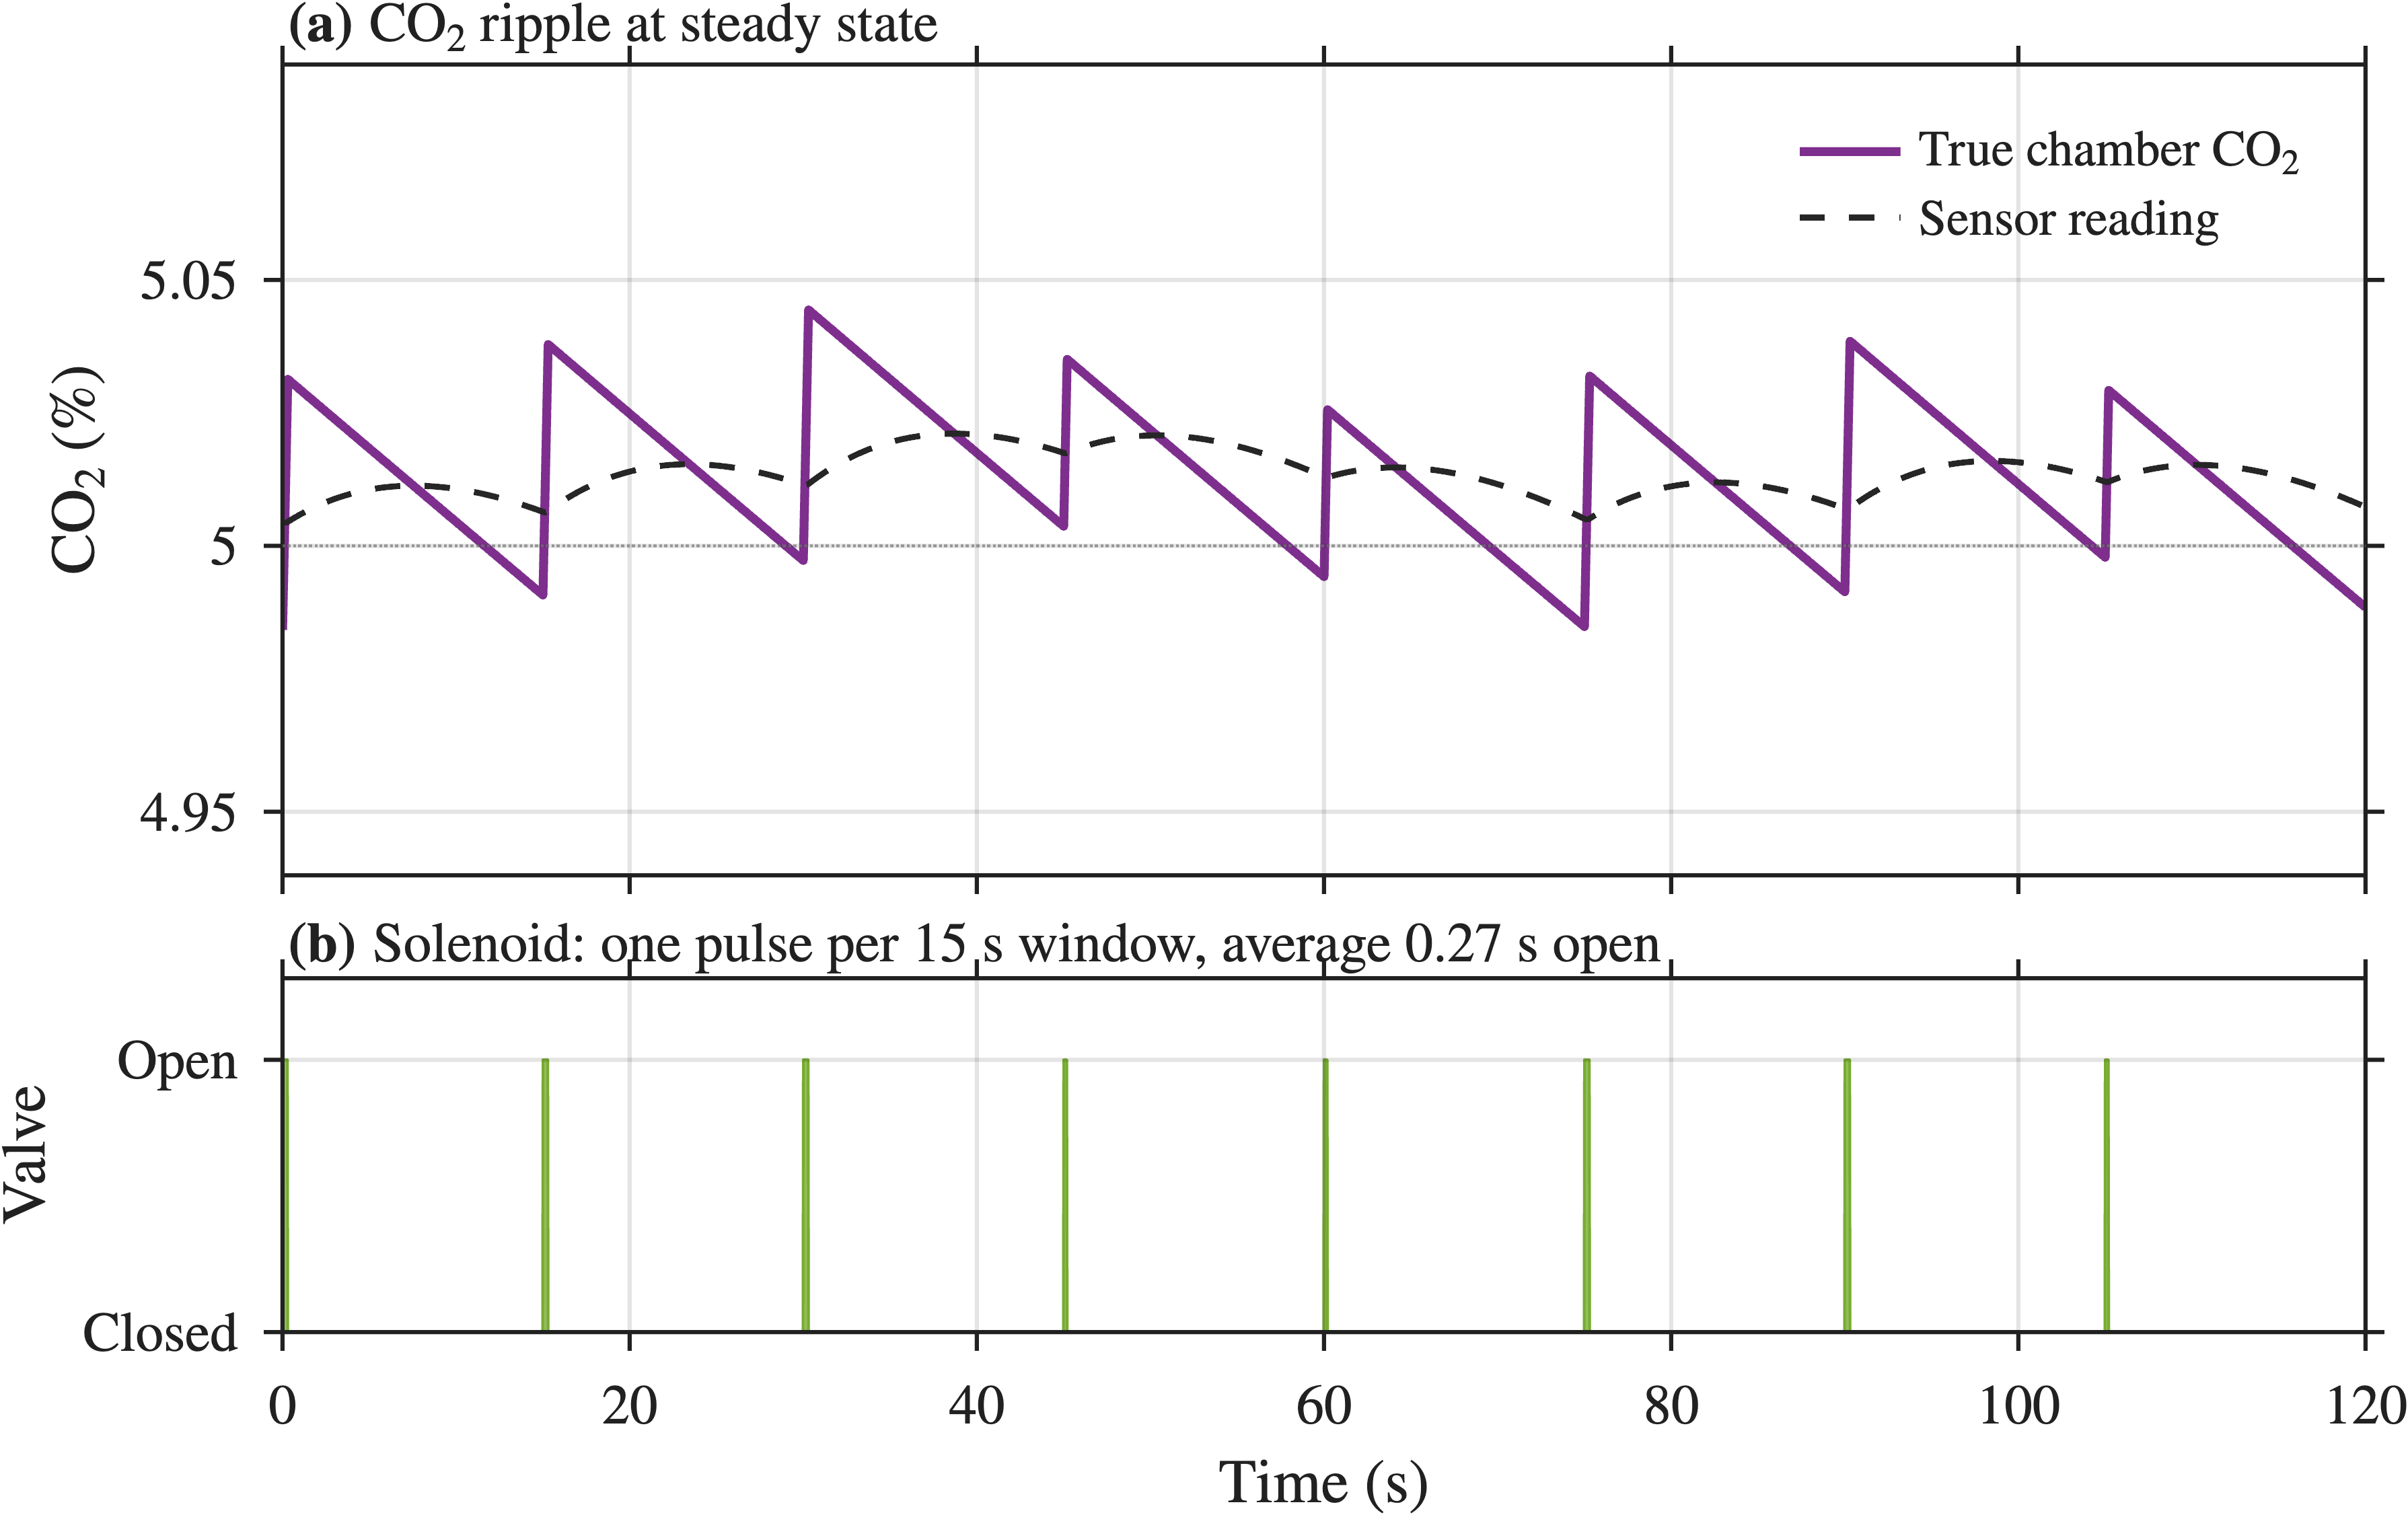
\includegraphics[width=0.74\textwidth,height=0.62\textheight,keepaspectratio]{figs/Control Simulation Figures/fig_C6_valve_pulses.png}
    \caption[Valve pulses at steady state]{\textbf{Valve pulses at steady state,} for the 0.99\,L design volume. The valve opens for about 0.27\,s once per 15\,s window, and each opening raises the concentration by about 0.04\,pp, giving a ripple of about 0.06\,pp. The shortest 0.1\,s pulse would add 0.016\,pp.}
    \label{fig_C6_valve_pulses}
\end{figure}

\begin{figure}[htbp]
    \centering
    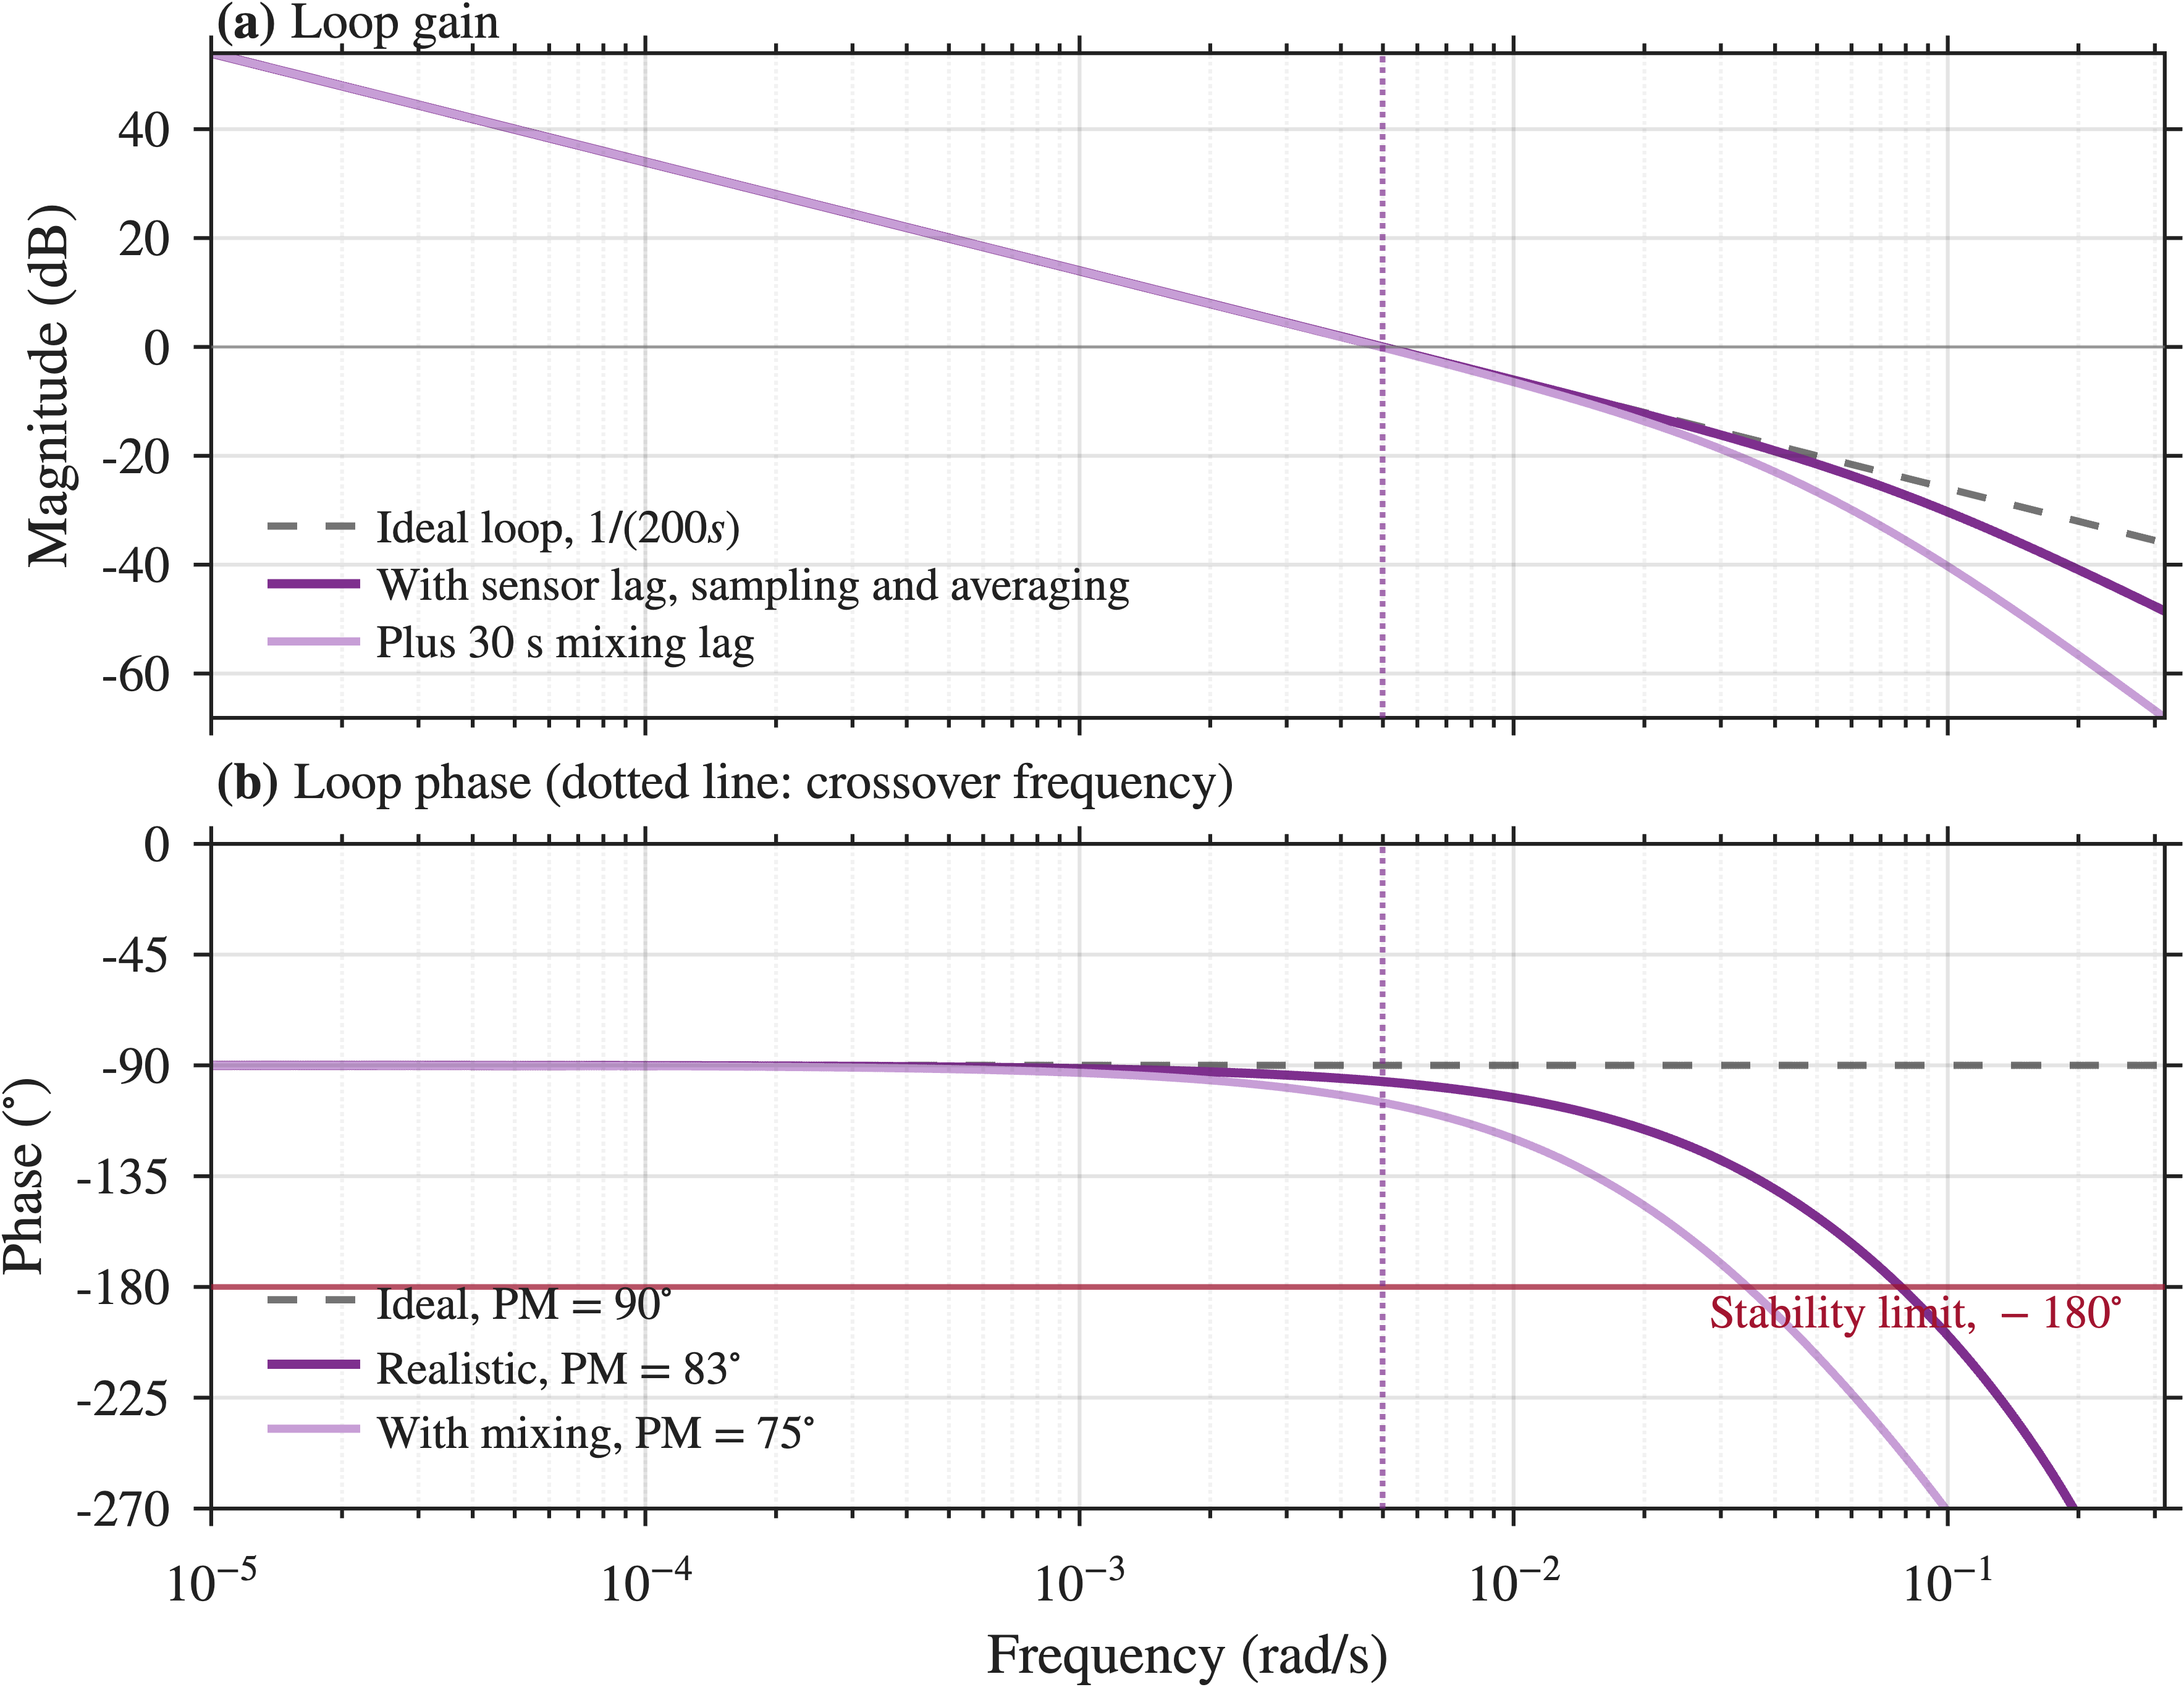
\includegraphics[width=0.74\textwidth,height=0.62\textheight,keepaspectratio]{figs/Control Simulation Figures/fig_C7_bode.png}
    \caption[Open-loop frequency response of the CO\textsubscript{2} loop]{\textbf{Open-loop frequency response of the CO\textsubscript{2} loop,} ideal, with the sensor lag and sampling, and with an added 30\,s mixing lag.}
    \label{fig_C7_bode}
\end{figure}
